\chapter{Theoretische und technische Grundlagen}

Im Rahmen dieses Kapitels werden die maßgeblichen Technologien und Konzepte dargelegt, auf denen das entwickelte Modell basiert. Der Fokus liegt auf der automatisierten Objekterkennung, Textextraktion und strukturierten Informationsverarbeitung aus Gleisplänen.
\section{Grafische Gleispläne im Bahnkontext}
Die Modellierung eines Bahnhofs stellt eine komplexe Aufgabe dar, da ein solcher in der Regel aus Hunderten von Gleisen und Weichen sowie zahlreichen Signalen besteht. 
Die manuelle Erstellung eines Bahnhofsmodells, das den physischen Details eines Bahnhofs entspricht, erfordert in der Regel mehrere Wochen Arbeit. Dies hat signifikante 
Auswirkungen auf die Anwendbarkeit und den Umfang vieler Methoden.\cite{railroadstationdrawing}


Diese zeitintensive manuelle Arbeit motiviert den Einsatz automatisierter Verfahren zur Datenextraktion. Die folgenden Abschnitte legen die theoretischen Grundlagen dar, auf denen eine solche Automatisierung aufbauen kann.

\subsection{Grundlagen des Gleisplans}
Der Gleisplan bildet die fundamentale Datengrundlage für die Planung, den Bau und den operativen Betrieb von Bahnanlagen. Er repräsentiert die technische Infrastruktur und dient als visuelle Schnittstelle zwischen der physischen Außenanlage und der sicherungstechnischen Logik (Stellwerk).
\\
Gleispläne existieren in zwei Darstellungsformen \cite{Pachl}: maßstäbliche 
Lagepläne (topografisch, bautechnisch) und schematische Übersichtspläne 
(topologisch, sicherungstechnisch). Diese Arbeit fokussiert letztere, da sie 
die logischen Fahrwegbeziehungen priorisieren und die Grundlage für die Stellwerksplanung bilden.

Gleispläne enthalten drei Symbolkategorien: (1) Fahrwegelemente (Gleise, Weichen), 
(2) Sicherungstechnik (Signale, Achszähler), (3) Metadaten (Bezeichner, 
Kilometrierung). Jedes Element trägt eindeutige Labels zur Identifikation.

Obwohl diese Pläne in der heutigen Ingenieurspraxis mittels CAD-Systemen (Computer Aided Design) erstellt werden, liegt die primäre Herausforderung für eine automatisierte Auswertung nicht im Dateiformat, sondern in der korrekten semantischen Interpretation dieser abstrahierten Symbolik und ihrer logischen Verknüpfung \cite{Pachl}.

\begin{figure}[h]
    \centering
    \includegraphics[width=1\textwidth]{images/gleisplandrawio.png} 
    \caption{Ausschnitt eines schematischen Gleisplans mit Darstellung von Signalen, Weichen und Gleisbezeichnungen (Beispielhafte Darstellung) aus Quelle \cite{railroadstationdrawing}}
    \label{fig:gleisplan_schema}
\end{figure}

\subsection{Bahntechnische Symbole und ihre Klassifikation}
\label{sec:Bahntechnischesymbole}
In den Gleisplänen kommen zahlreiche Symbole zum Einsatz, um die verschiedenen technischen Objekte, Anlagenkomponenten und zusätzlichen Informationen übersichtlich darzustellen. Diese Symboldarstellung dient nicht nur der Visualisierung der Gleiskomponenten, sondern bildet auch die Grundlage für Planung, Projektierung, Dokumentation und spätere Anwendung. \cite{signallayout} Da der Gleisplan eine zentrale Schnittstelle zwischen technischer Planung, 
betrieblicher Umsetzung und sicherheitstechnischen Systemen darstellt, ist eine präzise, klare und einheitliche Symbolklassifizierung notwendig. Die für diese Arbeit relevanten Symbolklassen gliedern sich in drei funktionale 
Kategorien (siehe Tabelle \ref{tab:symbol_categories}):

\begin{table}[h]
\centering
\begin{tabular}{|p{3cm}|p{12cm}|}
\hline
\textbf{Kategorie} & \textbf{Elemente und Funktion} \\
\hline
Infrastruktur & \textbf{Signale}: Fahrterlaubnis und Geschwindigkeitsvorgabe. 
\textbf{Weichen}: Fahrwegverzweigungen. \textbf{Isolierstöße}: Elektrische 
Gleistrennung. \textbf{Achszähler}: Belegungserkennung. \\
\hline
Zugbeeinflussung & \textbf{Balisen}: Punktförmige Datenübertragung an Zug. 
\textbf{Gleismagnete}: Induktive Informationsübertragung. \textbf{Gleiskoppelspulen}: 
Elektromagnetische Kopplung. \\
\hline
Metadaten & \textbf{Positionsangaben}: Kilometrierung, Lagepunkte. 
\textbf{Gleisabschnittsnamen}: Eindeutige Gleisidentifikation. \\
\hline
\end{tabular}
\caption{Klassifikation bahntechnischer Symbole}
\label{tab:symbol_categories}
\end{table}

Die detaillierte visuelle Darstellung dieser Symbole erfolgt in Abschnitt 4.1.
\section{Objekterkennung in Bildern}
\label{sec:objekterkennung}

Die automatisierte Analyse visueller Informationen bildet das Fundament zahlreicher technischer Anwendungen von der Qualitätskontrolle in der industriellen Fertigung über die medizinische Bildanalyse bis hin zur autonomen Navigation. Während Menschen mühelos in der Lage sind, Objekte in Bildern zu identifizieren und zu lokalisieren, erfordert die Replikation dieser Fähigkeit in Maschinen die Lösung komplexer Teilprobleme. Historisch wurde diese Aufgabe durch explizite Programmierung von Erkennungsregeln adressiert. Der konzeptionelle Durchbruch gelang durch maschinelles Lernen, insbesondere durch tiefe neuronale Netze, die relevante Merkmale selbstständig aus Trainingsdaten extrahieren können \cite{LeCun1998_GradientBasedLearning,Krizhevsky2012_AlexNet}.

Für technische Anwendungen wie die Analyse von Konstruktionszeichnungen oder Gleisplänen manifestieren sich spezifische Herausforderungen, die über die Verarbeitung natürlicher Fotografien hinausgehen. Im Folgenden werden zunächst die domänenspezifischen Anforderungen technischer Zeichnungen erläutert, bevor die grundlegenden methodischen Ansätze der Objekterkennung systematisch hergeleitet werden. Das Kapitel folgt dabei einer Progression vom Allgemeinen zum Spezifischen: Ausgehend von universellen Erkennungsprinzipien wird schrittweise die Anwendung auf bahntechnische Gleispläne konkretisiert.

\subsection{Objekterkennung in technischen CAD-Zeichnungen}
\label{subsec:cad_spezifisch}

Im Gegensatz zu natürlichen Szenen weisen technische Konstruktionszeichnungen spezifische Charakteristika auf, die dedizierte Lösungsansätze erfordern. Diese domänenspezifischen Besonderheiten haben direkten Einfluss auf die Wahl geeigneter Erkennungsverfahren und definieren die in Kapitel \ref{chap:anforderungen} formulierten funktionalen Anforderungen an das System.

\subsubsection{Domänenspezifische Eigenschaften}

Technische Zeichnungen unterscheiden sich fundamental von natürlichen Bildern in ihrer Entstehung und Struktur. CAD-Systeme (Computer-Aided Design) erzeugen vektorbasierte Repräsentationen, die geometrische Primitive wie Linien, Kreise und Polylinien sowie zugeordnete Metadaten enthalten. Die Konvertierung in Rasterformate (PDF, PNG) für ML-basierte Analyse führt jedoch zu einem Informationsverlust hinsichtlich topologischer Beziehungen und semantischer Layer-Informationen. Topologische Beziehungen beschreiben die Verbindungsstruktur zwischen Elementen -- etwa welche Gleisabschnitte durch eine Weiche verbunden sind oder welches Signal zu welchem Gleis gehört. Semantische Layer-Informationen kodieren die funktionale Zuordnung von Objekten zu Kategorien wie Gleisführung, Signaltechnik oder Oberleitung. Bei der Rasterisierung werden diese Strukturinformationen eliminiert; das Bild wird zu einer Ansammlung von Pixeln ohne inhärente Bedeutung. Diese Transformation von strukturierten zu unstrukturierten Daten motiviert den Einsatz von Deep-Learning-Verfahren, die robuste Mustererkennung auch ohne explizite topologische Information ermöglichen.

Bahntechnische Symbole folgen standardisierten Bibliotheken gemäß EN-Normen oder kundenspezifischen Richtlinien. Die Variabilität innerhalb einer Symbolklasse ist somit deutlich geringer als bei natürlichen Objekten wie Fahrzeugen oder Personen, jedoch erschweren kundenspezifische Anpassungen die Generalisierung über verschiedene Planungsunternehmen hinweg. Ein durchschnittlicher Bahnhofsgleisplan enthält zwischen 500 und 2000 individuelle Symbole auf einer Fläche von wenigen Quadratmetern, was eine deutlich höhere Objektdichte als in typischen Computer-Vision-Benchmark-Datensätzen wie COCO \cite{Lin2014_COCO} oder Pascal VOC \cite{Everingham2010_PascalVOC} darstellt. Zum Vergleich: COCO-Bilder enthalten im Durchschnitt 7 bis 10 Objekte, während ein Gleisplanausschnitt von vergleichbarer Pixelgröße 50 bis 100 Symbole aufweisen kann.

Anders als bei Objekten mit kanonischer Orientierung -- etwa Straßenverkehrsschilder (typischerweise frontal) oder Fußgänger (vertikal stehend) -- können bahntechnische Symbole und Textannotationen entlang der Gleisachsen in beliebigen Winkeln orientiert sein. Ein Weichensymbol kann beispielsweise in 16 verschiedenen Rotationen auftreten, die jeweils 22,5° Schritte zwischen 0° und 360° abdecken. Signale werden parallel zur Gleisachse positioniert, Gleisnummern folgen der Krümmung des Gleises. Diese Rotationsvariabilität ohne bevorzugte Ausrichtung erfordert rotationsinvariante Detektionsarchitekturen, deren Notwendigkeit in Abschnitt \ref{sec:obb} detailliert erläutert wird.

\subsubsection{Stand der Forschung}

Die Anwendung von Machine Learning auf technische Zeichnungen ist ein aktives Forschungsfeld mit Anwendungen in verschiedenen Ingenieurdisziplinen. Ahmed et al. \cite{Ahmed2011} entwickelten frühe Ansätze zur automatischen Segmentierung von architektonischen Grundrissen unter Verwendung morphologischer Operationen und Hough-Transformation. Moreno-García et al. \cite{Moreno2019} entwickelten ein umfassendes Framework zur Digitalisierung komplexer technischer Zeichnungen und demonstrierten die Überlegenheit von Deep-Learning-Ansätzen gegenüber klassischen Feature-Engineering-Methoden. Rahul et al. \cite{Rahul2019} extrahierten Informationen aus P\&ID-Diagrammen der Prozessindustrie mittels Faster R-CNN und erreichten dabei mean Average Precision-Werte von über 85\%.

Jamieson et al. \cite{Jamieson2024} liefern eine umfassende Übersicht über Deep-Learning-Methoden für Engineering-Diagramme und identifizieren als zentrale Herausforderungen die hohe Variabilität kundenspezifischer Symbolbibliotheken, den Mangel an annotierten Trainingsdaten sowie die Notwendigkeit rotationsinvarianter Detektionsverfahren. Für den bahntechnischen Bereich existieren bisher hauptsächlich proprietäre Lösungen einzelner Eisenbahnunternehmen ohne publizierte wissenschaftliche Evaluierung. Die vorliegende Arbeit adressiert diese Forschungslücke durch Entwicklung und Evaluation eines prototypischen Systems auf Basis moderner One-Stage-Detektoren.

\subsection{Paradigmen der Objekterkennung}
\label{subsec:paradigmen}

Die historische Entwicklung der Objekterkennung lässt sich in drei methodische Hauptströmungen unterteilen, die sich hinsichtlich ihrer theoretischen Fundierung und praktischen Anwendbarkeit signifikant unterscheiden \cite{Zou2019_ObjectDetectionSurvey,Liu2020_DeepLearningDetectionSurvey}. Diese Evolution reflektiert den Übergang von expliziter Programmierung über datengetriebenes Lernen hin zu hierarchischer Merkmalsrepräsentation.

\subsubsection{Regelbasierte Verfahren}

Frühe Ansätze basierten auf der Anwendung manuell entwickelter Algorithmen. Template Matching schiebt ein Referenzmuster pixelweise über das Zielbild und quantifiziert die Ähnlichkeit mittels Korrelationsmetriken \cite{Brunelli2009}. Fortgeschrittenere Varianten wie SIFT (Scale-Invariant Feature Transform) oder SURF (Speeded Up Robust Features) extrahieren lokale Merkmale mit gewisser Robustheit gegenüber Skalierungs- und Beleuchtungsvariationen \cite{Lowe2004,Bay2008}.

Die fundamentale Limitierung liegt in der mangelnden Generalisierungsfähigkeit. Da die Merkmalsdefinition a priori erfolgen muss, versagen diese Ansätze bei unvorhergesehenen Variationen. Für Gleispläne mit mehr als 13 Symbolklassen in beliebigen Rotationszuständen ist eine erschöpfende Enumeration aller Template-Varianten computationell nicht handhabbar. Ein Weichensymbol in 16 Rotationen bei 3 Maßstäben würde bereits 48 Templates erfordern; für 13 Klassen summiert sich dies auf über 600 Varianten. Zudem erfordern kundenspezifische Anpassungen der Symbolbibliothek eine manuelle Neudefinition der Templates.

\subsubsection{Maschinelles Lernen mit konstruierten Merkmalen}

Verfahren wie Support Vector Machines (SVM) \cite{Cortes1995_SVM} in Kombination mit Histogram of Oriented Gradients (HOG) Features \cite{Dalal2005} lernen Erkennungslogik aus Trainingsdaten. Der fundamentale Unterschied zu regelbasierten Ansätzen liegt in der Adaptivität: Das System lernt selbstständig relevante Merkmalskombinationen aus annotierten Beispielen. Dennoch verbleibt die Merkmalsextraktion (Feature Engineering) als manuelle Aufgabe. Ein Ingenieur muss entscheiden, welche Bildcharakteristika -- etwa Gradientenrichtungen, Farbhistogramme oder Texturstatistiken -- für die jeweilige Domäne relevant sind \cite{Lowe2004,Dalal2005}. Die Güte des Gesamtsystems ist direkt an die Qualität dieser handdefinierten Merkmalsrepräsentation gekoppelt. Bei technischen Zeichnungen mit ihrer Kombination aus geometrischer Präzision, variabler Linienstärke und dichtem Layout erreichen diese Verfahren schnell ihre Leistungsgrenzen.

\subsubsection{Deep Learning und End-to-End-Lernen}

Moderne Ansätze basieren auf Convolutional Neural Networks (CNNs), die hierarchische Repräsentationen direkt aus Rohdaten lernen \cite{LeCun1998_GradientBasedLearning,Krizhevsky2012_AlexNet}. Das fundamentale Designprinzip ist die automatische Merkmalsentdeckung: Anstelle expliziter Regeln oder vordefinierter Feature-Deskriptoren extrahiert das Netz Features selbstständig durch wiederholte Anwendung von Faltungsoperationen. 

Die Funktionsweise basiert auf hierarchischer Merkmalskomposition. Die ersten Schichten eines CNN reagieren auf einfache visuelle Muster wie Linien in unterschiedlichen Orientierungen. Diese werden durch kleine Faltungsfilter (typischerweise 3×3 oder 5×5 Pixel) detektiert \cite{Zeiler2014_Visualizing}. Höhere Schichten kombinieren diese Basismuster zu komplexeren Strukturen: aus Linien werden Ecken und Kurven, aus diesen werden geometrische Formen, und schließlich emergieren symbolspezifische Muster wie die charakteristische T-Form einer Weiche oder die kreisförmige Struktur eines Signals. Das Netz lernt diese Hierarchie selbstständig, indem es während des Trainings annotierte Beispiele analysiert und seine internen Parameter (Filtergewichte) so anpasst, dass Vorhersagefehler minimiert werden \cite{LeCun1998_GradientBasedLearning}.

Abbildung \ref{fig:cnn_feature_hierarchy} verdeutlicht diese progressive Abstraktion. Die erste Schicht detektiert lediglich Linienorientierungen mittels kleiner 3×3 Filter. Die zweite Schicht kombiniert diese Basismuster zu geometrischen Elementen wie Ecken, Kurven und Kreisen. In der dritten Schicht entstehen komplexere Formen wie Rechtecke, T-Formen und Pfeile. Schließlich emergieren in der finalen Schicht symbolspezifische Repräsentationen wie Weichen, Signale oder Gleisabschnitte. Diese zunehmende Komplexität der Features wird durch wiederholte Faltungsoperationen erreicht, wobei jede Schicht auf den Ausgaben der vorherigen aufbaut.

\begin{figure}[H]
\centering
\begin{tikzpicture}[
    node distance=0.8cm and 1.2cm,
    % STYLES
    layer/.style={
        rectangle, draw, thick, 
        minimum width=2.0cm, minimum height=4.0cm, 
        align=center
    },
    feature/.style={
        rectangle, draw, 
        minimum width=1.6cm, minimum height=0.6cm, 
        align=center, font=\tiny,
        fill=white!90!gray, 
        drop shadow 
    },
    layer_title/.style={font=\bfseries\scriptsize, align=center},
    layer_sub/.style={font=\tiny, align=center, color=black!70},
    arrow/.style={->, >=stealth, thick}
]

    % ==========================
    % 1. INPUT (Kleiner als die anderen)
    % ==========================
    \node[layer, fill=blue!15, minimum height=3cm] (input) {};
    \node[above=0.2cm of input.center] (in_img) {
        \tikz{\draw[thick, fill=white] (0,0) rectangle (0.8,0.8); \draw[thick, red] (0.4,0.4) circle (0.2);}
    };
    \node[above=0.1cm of in_img, font=\small] {Eingabe};
    \node[below=0.1cm of in_img, font=\tiny, align=center] {Gleisplan\\1024$\times$1024};

    % ==========================
    % 2. LAYER 1
    % ==========================
    \node[layer, fill=yellow!20, right=of input] (layer1) {};
    \node[layer_title, below=0.1cm of layer1.north] (t1) {Schicht 1};
    \node[layer_sub, below=0.0cm of t1] (st1) {Einfache\\Muster};
    
    \node[feature, below=0.2cm of st1] (f1) {Horizontal};
    \node[feature, below=0.1cm of f1] (f2) {Vertikal};
    \node[feature, below=0.1cm of f2] (f3) {Diagonal};

    % ==========================
    % 3. LAYER 2
    % ==========================
    \node[layer, fill=orange!20, right=of layer1] (layer2) {};
    \node[layer_title, below=0.1cm of layer2.north] (t2) {Schicht 2};
    \node[layer_sub, below=0.0cm of t2] (st2) {Geometrie};
    
    \node[feature, below=0.2cm of st2] (f4) {Ecken};
    \node[feature, below=0.1cm of f4] (f5) {Kurven};
    \node[feature, below=0.1cm of f5] (f6) {Kreise};

    % ==========================
    % 4. LAYER 3
    % ==========================
    \node[layer, fill=red!20, right=of layer2] (layer3) {};
    \node[layer_title, below=0.1cm of layer3.north] (t3) {Schicht 3};
    \node[layer_sub, below=0.0cm of t3] (st3) {Formen};
    
    \node[feature, below=0.2cm of st3] (f7) {Rechteck};
    \node[feature, below=0.1cm of f7] (f8) {T-Form};
    \node[feature, below=0.1cm of f8] (f9) {Pfeil};

    % ==========================
    % 5. OUTPUT
    % ==========================
    \node[layer, fill=green!20, right=of layer3] (output) {};
    \node[layer_title, below=0.1cm of output.north] (t4) {Ausgabe};
    \node[layer_sub, below=0.0cm of t4] (st4) {Symbole};
    
    \node[feature, below=0.2cm of st4] (s1) {Weiche};
    \node[feature, below=0.1cm of s1] (s2) {Signal};
    \node[feature, below=0.1cm of s2] (s3) {Gleis};

    % ==========================
    % ARROWS & LABELS
    % ==========================
    \draw[arrow] (input) -- (layer1);
    \draw[arrow] (layer1) -- (layer2);
    \draw[arrow] (layer2) -- (layer3);
    \draw[arrow] (layer3) -- (output);

    \node[above=0.1cm of layer1, font=\scriptsize] {3$\times$3 Filter};
    \node[above=0.1cm of layer2, font=\scriptsize] {Kombination};
    \node[above=0.1cm of layer3, font=\scriptsize] {Abstraktion};

    % --- HIER IST DER FIX ---
    % Wir nutzen (input |- output.south): X von Input, Y von Output.south
    \draw[->, >=stealth, very thick, blue!60!black] 
        ([yshift=-0.5cm] input |- output.south) -- ([yshift=-0.5cm] output.south)
        node[midway, below, font=\small] {Zunehmende Komplexität der Features};

\end{tikzpicture}
\caption{Hierarchische Merkmalsextraktion in Convolutional Neural Networks.}
\label{fig:cnn_feature_hierarchy_straight}
\end{figure}
Diese End-to-End-Lernfähigkeit ermöglicht eine Robustheit, die mit konventionellen Verfahren nicht erreichbar ist. Für technische Zeichnungen erweisen sich Deep-Learning-Architekturen als überlegen, da sie sowohl exakte Lokalisierung als auch semantische Klassifikation integriert durchführen können, ohne dass ein Ingenieur domänenspezifische Features manuell definieren muss \cite{Girshick2014_RCNN,Ren2015_FasterRCNN}.

\subsection{Architekturen für Deep-Learning-basierte Objekterkennung}
\label{subsec:dl_architekturen}

Die Implementierung von CNN-basierten Objektdetektoren lässt sich in zwei Architekturparadigmen unterteilen, die sich in ihrer Balance zwischen Detektionsgenauigkeit und Recheneffizienz unterscheiden. Die Wahl der Architektur hat direkte Auswirkungen auf die Praxistauglichkeit des Systems.

\subsubsection{Zweistufige vs. einstufige Detektoren}

Zweistufige Detektoren wie Faster R-CNN \cite{Ren2015_FasterRCNN} separieren den Erkennungsprozess konzeptionell in zwei aufeinanderfolgende Phasen. Zunächst generiert ein Region Proposal Network (RPN) zwischen 100 und 300 Kandidatenregionen, die potenziell Objekte enthalten könnten. Diese Regionen werden anschließend durch ein separates Klassifikationsnetzwerk evaluiert, das sowohl die Objektklasse bestimmt als auch die Bounding-Box-Koordinaten verfeinert. Der Vorteil liegt in hoher Detektionspräzision, insbesondere bei kleinen oder teilweise verdeckten Objekten. Die sequenzielle Verarbeitung hunderter Kandidatenregionen führt jedoch zu Bildraten von lediglich 5 bis 10 Bildern pro Sekunde (Frames Per Second, FPS) auf moderner GPU-Hardware (Graphics Processing Unit).

Für die Gleisplananalyse erweist sich diese Geschwindigkeit als kritisch. Ein durchschnittlicher Plan umfasst nach der Kachelungsstrategie (siehe Abschnitt \ref{subsec:tiling_strategie}) zwischen 150 und 300 Bildausschnitte. Während YOLO-Modelle typischerweise mit Eingangsgrößen von 640×640 oder 1024×1024 Pixeln arbeiten, werden für die Gleisplananalyse aufgrund der sehr kleinen Symbolgrößen Kacheln von 2048×2048 Pixeln verwendet (Details zur Kachelungsstrategie in Abschnitt \ref{subsec:tiling_strategie}). Bei einer Verarbeitungszeit von 100 bis 200 Millisekunden pro Kachel würde die Gesamtanalyse zwischen 15 Sekunden und 4 Minuten dauern. Dies widerspricht der in Kapitel \ref{chap:anforderungen} definierten Anforderung einer interaktiven Benutzeroberfläche, die Analyseergebnisse innerhalb von maximal 10 Sekunden präsentieren soll.

Einstufige Detektoren wie YOLO (You Only Look Once) \cite{redmon2016lookonceunifiedrealtime} adressieren diese Geschwindigkeitsproblematik durch eine fundamental andere Strategie. YOLO unterteilt das Eingabebild in ein regelmäßiges Raster von Zellen (beispielsweise 13×13 oder 26×26 Zellen bei kleineren Eingabegrößen, bzw. entsprechend größere Raster bei höheren Auflösungen). Für jede Zelle sagt das Netz in einem einzigen Vorwärtsdurchlauf direkt mehrere Aspekte voraus: Liegt in dieser Zelle ein Objekt? Wenn ja, welcher Objektklasse gehört es an? Wie hoch ist die Konfidenz dieser Vorhersage? Und wo genau innerhalb der Zelle befindet sich das Objekt? Diese parallele Verarbeitung aller Bildbereiche ermöglicht Inferenzgeschwindigkeiten von 40 bis über 100 Bildern pro Sekunde \cite{yolov8_ultralytics}. Moderne Varianten wie YOLOv8 erreichen durch architektonische Verbesserungen -- insbesondere Feature Pyramid Networks (FPN) \cite{Lin2017_FPN} für Multi-Scale-Detektion und verbesserte Loss-Funktionen -- vergleichbare oder sogar überlegene Präzision gegenüber zweistufigen Detektoren bei Beibehaltung der Echtzeitfähigkeit.

Die Abwägung zwischen beiden Paradigmen muss im Kontext der Anwendungsanforderungen erfolgen. Für technische Gleispläne mit gut sichtbaren, scharf gerenderten Symbolen rechtfertigt die hohe Verarbeitungsgeschwindigkeit marginale Genauigkeitseinbußen. Die in Kapitel \ref{chap:evaluation} dargestellten Ergebnisse bestätigen, dass eine mean Average Precision von über 98\% mit einstufigen Architekturen erreichbar ist, bei gleichzeitiger Gesamtverarbeitungszeit von etwa 5 Sekunden pro Plan.

Abbildung \ref{fig:two_stage_vs_one_stage} illustriert den fundamentalen Unterschied zwischen beiden Architekturparadigmen. Faster R-CNN generiert zunächst mehrere hundert Kandidatenregionen mittels RPN, die anschließend sequenziell klassifiziert werden müssen. YOLO hingegen sagt in einem einzigen Vorwärtsdurchlauf direkt die Bounding Boxes und Klassen voraus, was zu einer Beschleunigung um den Faktor 5 führt. Für die Analyse eines typischen Gleisplans mit 200 gekachelten Bildausschnitten (je 2048×2048 Pixel) reduziert sich die Gesamtverarbeitungszeit von etwa 4 Minuten (Faster R-CNN) auf unter 5 Sekunden (YOLO).

% ABBILDUNG 3.2: Two-Stage vs One-Stage
\begin{figure}[H]
\centering
\begin{tikzpicture}[
    node distance=1.5cm,
    box/.style={rectangle, draw, thick, minimum width=2.8cm, minimum height=1cm, align=center, font=\footnotesize},
    arrow/.style={->, >=stealth, thick}
]
    % LEFT: Two-Stage
    \node[box, fill=blue!15] (img1) {Eingabebild\\$1024 \times 1024$ px};
    \node[box, fill=yellow!25, below=of img1] (rpn) {Region Proposal\\Network\\$\sim$300 Kandidaten};
    \node[box, fill=orange!20, below=of rpn] (class1) {Klassifikation\\pro Region};
    \node[box, fill=green!20, below=of class1] (out1) {Detektionen};
    
    \draw[arrow] (img1) -- (rpn);
    \draw[arrow] (rpn) -- (class1);
    \draw[arrow] (class1) -- (out1);
    
    \node[left=0.6cm of rpn, align=right, font=\scriptsize\bfseries] (label1) {Two-Stage\\(Faster R-CNN)};
    \node[below=0.15cm of label1, align=right, font=\tiny, text width=2.2cm] {$\sim$8 FPS\\Hohe Präzision\\4 Min/Gleisplan};
    
    % RIGHT: One-Stage
    \begin{scope}[xshift=6.5cm]
        \node[box, fill=blue!15] (img2) {Eingabebild\\$1024 \times 1024$ px};
        \node[box, fill=green!20, below=3.2cm of img2] (direct) {Direkte Vorhersage\\(Grid-basiert)};
        \node[box, fill=green!20, below=of direct] (out2) {Detektionen};
        
        \draw[arrow] (img2) -- (direct);
        \draw[arrow] (direct) -- (out2);
        
        \node[right=0.6cm of direct, align=left, font=\scriptsize\bfseries] (label2) {One-Stage\\(YOLO)};
        \node[below=0.15cm of label2, align=left, font=\tiny, text width=2.2cm] {$\sim$40 FPS\\Echtzeitfähig\\5 Sek/Gleisplan};
    \end{scope}
    
    % Comparison arrow
    \draw[<->, >=stealth, thick, red!70!black] (out1.south) ++ (0,-0.4) -- ++ (6.5,0) 
        node[midway, below, font=\scriptsize, align=center] {Faktor 5 schneller};
\end{tikzpicture}
\caption{Architekturvergleich zwischen zweistufigen und einstufigen Objektdetektoren.}
\label{fig:two_stage_vs_one_stage}
\end{figure}

\subsection{Training und Optimierung}
\label{subsec:training_optimization}

Die Leistungsfähigkeit neuronaler Netze hängt kritisch vom Trainingsprozess ab, durch den die internen Parameter (Gewichte) des Netzes aus annotierten Beispieldaten gelernt werden. Dieser Abschnitt erläutert die fundamentalen Mechanismen des Trainings und deren Implikationen für die Gleisplanerkennung.

\subsubsection{Supervised Learning und Loss-Funktionen}

Das Training erfolgt im Supervised-Learning-Paradigma \cite{Goodfellow2016_DeepLearning}: Dem Netz werden Eingabebilder zusammen mit korrekten Annotationen (Ground Truth) präsentiert. Für Objektdetektion umfassen diese Annotationen sowohl die Bounding-Box-Koordinaten als auch die Klassenbezeichnung jedes Objekts. Das Netz generiert Vorhersagen, die mit der Ground Truth verglichen werden. Die Diskrepanz wird durch eine Loss-Funktion quantifiziert, die typischerweise mehrere Komponenten kombiniert:

Der Klassifikations-Loss misst, wie gut die vorhergesagte Objektklasse mit der tatsächlichen Klasse übereinstimmt. Üblich ist die Cross-Entropy-Loss \cite{Goodfellow2016_DeepLearning}, die hohe Konfidenz für korrekte Klassen belohnt und niedrige Konfidenz für falsche Klassen fordert. Die Lokalisierungs-Loss quantifiziert die Abweichung zwischen vorhergesagter und tatsächlicher Bounding Box, häufig implementiert als Smooth L1-Loss über die Box-Koordinaten \cite{Ren2015_FasterRCNN}. Moderne Detektoren wie YOLOv8 verwenden zusätzlich IoU-basierte Loss-Komponenten \cite{Rezatofighi2019_GIoU}, die direkt den Überlappungsgrad optimieren anstatt nur Koordinatenabweichungen zu minimieren.

Der Trainingsprozess iteriert über den Datensatz in kleinen Batches (typischerweise 8 bis 32 Bilder). Für jedes Batch wird der Loss berechnet und mittels Backpropagation \cite{Rumelhart1986_Backpropagation} -- einem effizienten Algorithmus zur Berechnung von Gradienten -- ermittelt, wie jedes Gewicht im Netz angepasst werden muss, um den Loss zu reduzieren. Ein Optimierer wie SGD (Stochastic Gradient Descent) \cite{Robbins1951_SGD} oder Adam \cite{Kingma2015_Adam} führt diese Gewichtsanpassungen durch. Die Lernrate steuert die Schrittgröße dieser Anpassungen; typische Werte liegen zwischen 0.001 und 0.01. Das Training erstreckt sich über mehrere hundert Epochen, wobei eine Epoche einen vollständigen Durchlauf durch alle Trainingsdaten bezeichnet.

Abbildung \ref{fig:training_loop} visualisiert diesen iterativen Prozess. Ein Batch von Trainingsbildern wird zunächst durch das Netz propagiert (Forward Pass), wobei für jedes Bild Vorhersagen generiert werden. Diese Vorhersagen werden mit den korrekten Annotationen verglichen, und die Diskrepanz wird als Loss quantifiziert. Mittels Backpropagation werden anschließend die Gradienten für alle Gewichte berechnet. Der Optimizer nutzt diese Gradienten, um die Gewichte schrittweise anzupassen. Dieser Zyklus wiederholt sich für jeden Batch im Datensatz. Nach einem vollständigen Durchlauf durch alle Trainingsdaten (eine Epoche) beginnt die nächste Epoche. Das Training konvergiert typischerweise nach mehreren hundert Epochen, wobei der Loss kontinuierlich abnimmt.

% ABBILDUNG 3.4: Training Loop
\begin{figure}[H]
\centering
\begin{tikzpicture}[
    node distance=1.2cm,
    box/.style={rectangle, draw, thick, minimum width=3cm, minimum height=1cm, align=center, font=\small},
    roundbox/.style={rectangle, rounded corners, draw, thick, minimum width=3cm, minimum height=1cm, align=center, font=\small},
    arrow/.style={->, >=stealth, thick}
]
    % Training Data
    \node[box, fill=blue!15] (data) {Trainingsdaten\\Bilder + Annotationen};
    
    % Forward Pass
    \node[box, fill=yellow!20, below=of data] (forward) {Forward Pass\\Vorhersagen generieren};
    
    % Loss Calculation
    \node[box, fill=orange!20, below=of forward] (loss) {Loss-Berechnung\\Fehler quantifizieren};
    
    % Backpropagation
    \node[roundbox, fill=red!20, below=of loss] (backprop) {Backpropagation\\Gradienten berechnen};
    
    % Weight Update
    \node[roundbox, fill=green!20, below=of backprop] (update) {Gewichte anpassen\\Optimizer (SGD/Adam)};
    
    % Arrows
    \draw[arrow] (data) -- (forward);
    \draw[arrow] (forward) -- (loss);
    \draw[arrow] (loss) -- (backprop);
    \draw[arrow] (backprop) -- (update);
    
    % Loop back
    \draw[arrow, dashed, thick, blue!60!black] (update.east) -- ++(1.5,0) |- (forward.east)
        node[midway, right, align=left, font=\scriptsize] {Nächster\\Batch};
    
    % Side annotations
    \node[left=0.8cm of forward, align=right, font=\scriptsize, text width=2.5cm] 
        {CNN generiert\\Bounding Boxes\\+ Klassen};
    \node[left=0.8cm of loss, align=right, font=\scriptsize, text width=2.5cm] 
        {Vergleich mit\\Ground Truth\\$\mathcal{L} = \mathcal{L}_{\text{cls}} + \mathcal{L}_{\text{loc}}$};
    \node[left=0.8cm of backprop, align=right, font=\scriptsize, text width=2.5cm] 
        {$\frac{\partial \mathcal{L}}{\partial w_i}$\\für alle Gewichte};
    \node[left=0.8cm of update, align=right, font=\scriptsize, text width=2.5cm] 
        {$w_i \leftarrow w_i - \eta \frac{\partial \mathcal{L}}{\partial w_i}$};
    
    % Epoch indicator
    \node[below=1.5cm of update, font=\small, align=center] 
        {Wiederholung über mehrere hundert Epochen\\bis Konvergenz};
\end{tikzpicture}
\caption{Trainingszyklus eines CNN-basierten Objektdetektors.}
\label{fig:training_loop}
\end{figure}

\subsubsection{Data Augmentation und Generalisierung}

Eine zentrale Herausforderung beim Training neuronaler Netze ist Overfitting \cite{Goodfellow2016_DeepLearning}: Das Netz memoriert die Trainingsbeispiele anstatt generalisierbare Muster zu lernen. Datenerweiterung (Data Augmentation) \cite{dataugmentation} adressiert dieses Problem durch künstliche Erhöhung der Datensatzvielfalt. Während des Trainings werden Bilder on-the-fly transformiert durch Operationen wie horizontales Spiegeln, Rotation, Skalierung, Helligkeitsanpassung oder Hinzufügen von Rauschen. Für Gleispläne ist insbesondere Rotation essenziell, da Symbole in beliebigen Orientierungen auftreten können. Mosaic Augmentation \cite{Bochkovskiy2020_YOLOv4}, eine Technik, die vier Trainingsbilder zu einem zusammenfügt, erhöht zusätzlich die Robustheit gegenüber variablen Objektdichten.

Abbildung \ref{fig:data_augmentation} zeigt typische Augmentation-Techniken im Überblick. Ein Originalbild wird während des Trainings zufällig transformiert. Rotation um ±30° simuliert die beliebige Orientierung von Symbolen in Gleisplänen. Horizontale Spiegelung verdoppelt effektiv die Datensatzgröße ohne zusätzliche Annotation. Skalierung zwischen 0.8× und 1.2× erhöht die Robustheit gegenüber variierenden Symbolgrößen. Helligkeitsanpassung um ±20\% kompensiert unterschiedliche Scan- oder Digitalisierungsqualitäten. Mosaic Augmentation kombiniert vier Trainingsbilder zu einem einzigen Bild und erhöht die Exposition gegenüber hohen Objektdichten -- besonders relevant für Gleispläne mit bis zu 100 Symbolen pro Bildausschnitt. Diese Transformationen werden on-the-fly während des Trainings angewendet, sodass das Netz in jeder Epoche leicht unterschiedliche Versionen derselben Trainingsbilder sieht.

\begin{figure}[H]
\centering
\begin{tikzpicture}[
    node distance=0.8cm and 0.4cm,
    imgbox/.style={
        rectangle, 
        draw, 
        thick, 
        minimum width=3.2cm, 
        minimum height=2.8cm, 
        align=center, 
        font=\scriptsize
    },
    % HIER IST DIE ÄNDERUNG: \boldmath hinzugefügt
    label/.style={font=\scriptsize\bfseries\boldmath}
]

    % --- REIHE 1 ---

    % 1. Original
    \node[imgbox, fill=blue!10] (orig) {Original\\[0.2cm]
    \begin{tikzpicture}[scale=0.5]
        \draw[very thick, fill=white] (0,0) rectangle (2,1);
        \draw[very thick, red] (0.5,0.5) circle (0.3);
        \draw[thick] (1.5, 0.2) -- (1.5, 0.8);
    \end{tikzpicture}};
    \node[label, below=0.1cm of orig] (l_orig) {Original};
    
    % 2. Rotation
    \node[imgbox, fill=yellow!15, right=of orig] (rot) {Rotation\\[0.2cm]
    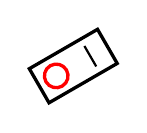
\begin{tikzpicture}[scale=0.5, rotate=30]
        \draw[very thick, fill=white] (0,0) rectangle (2,1);
        \draw[very thick, red] (0.5,0.5) circle (0.3);
        \draw[thick] (1.5, 0.2) -- (1.5, 0.8);
    \end{tikzpicture}};
    % Jetzt fett durch \boldmath im Style
    \node[label, below=0.1cm of rot] (l_rot) {$\pm 30^\circ$};
    
    % 3. Spiegelung
    \node[imgbox, fill=green!15, right=of rot] (flip) {Spiegelung\\[0.2cm]
    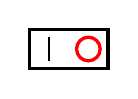
\begin{tikzpicture}[scale=0.5]
        \draw[very thick, fill=white] (0,0) rectangle (2,1);
        \draw[very thick, red] (1.5,0.5) circle (0.3);
        \draw[thick] (0.5, 0.2) -- (0.5, 0.8);
    \end{tikzpicture}};
    \node[label, below=0.1cm of flip] (l_flip) {Horizontal};
    
    
    % --- REIHE 2 ---
    
    % 4. Skalierung
    \node[imgbox, fill=orange!15, below=of l_orig] (scale) {Skalierung\\[0.2cm]
    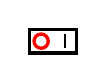
\begin{tikzpicture}[scale=0.3]
        \draw[very thick, fill=white] (0,0) rectangle (2,1);
        \draw[very thick, red] (0.5,0.5) circle (0.3);
        \draw[thick] (1.5, 0.2) -- (1.5, 0.8);
    \end{tikzpicture}};
    \node[label, below=0.1cm of scale] (l_scale) {0.5--1.5$\times$};
    
    % 5. Helligkeit
    \node[imgbox, fill=purple!15, right=of scale] (bright) {Helligkeit\\[0.2cm]
    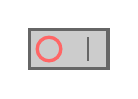
\begin{tikzpicture}[scale=0.5]
        \draw[very thick, black!60, fill=gray!40] (0,0) rectangle (2,1);
        \draw[very thick, red!60] (0.5,0.5) circle (0.3);
        \draw[thick, black!60] (1.5, 0.2) -- (1.5, 0.8);
    \end{tikzpicture}};
    % Jetzt fett durch \boldmath im Style
    \node[label, below=0.1cm of bright] (l_bright) {$\pm 20\%$};
    
    % 6. Mosaic
    \node[imgbox, fill=red!15, right=of bright] (mosaic) {Mosaic\\[0.2cm]
    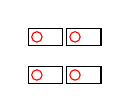
\begin{tikzpicture}[scale=0.22]
        \foreach \x/\y in {0/0, 2.2/0, 0/2.2, 2.2/2.2} {
            \draw[fill=white] (\x,\y) rectangle ++(2,1);
            \draw[red] (\x+0.5,\y+0.5) circle (0.3);
        }
    \end{tikzpicture}};
    \node[label, below=0.1cm of mosaic] (l_mosaic) {4 Bilder};
    
    
    % --- PFEIL ---
    \draw[->, >=stealth, very thick, blue!60!black] 
        ([yshift=-0.3cm]l_scale.south west) -- ([yshift=-0.3cm]l_mosaic.south east)
        node[midway, below, font=\small] {Data Augmentation während Training};

\end{tikzpicture}
\caption{Data Augmentation-Strategien: Vergrößerte Darstellung mit fetten Beschriftungen.}
\label{fig:data_augmentation_bold}
\end{figure}

Transfer Learning \cite{transferlearning} ist eine weitere Strategie zur Verbesserung der Generalisierung. Anstatt ein Netz von Grund auf zu trainieren, wird ein auf einem großen Datensatz (etwa ImageNet \cite{Deng2009_ImageNet} oder COCO \cite{Lin2014_COCO}) vortrainiertes Modell als Startpunkt verwendet. Die unteren Schichten, die generische Features wie Kanten und Texturen gelernt haben, werden beibehalten; lediglich die oberen Schichten werden auf die spezifische Domäne (Gleispläne) angepasst. Dies reduziert den Bedarf an domänenspezifischen Trainingsdaten signifikant \cite{NIPS2014_532a2f85}. Für die in Kapitel \ref{chap:implementation} beschriebene Implementierung wird YOLOv8 mit auf COCO vortrainierten Gewichten initialisiert und anschließend auf bahntechnischen Daten fine-tuned.

\subsection{Evaluationsmetriken}
\label{subsec:evaluationsmetriken}

Die Bewertung von Objektdetektoren erfordert standardisierte Metriken, die sowohl Lokalisierungsgenauigkeit als auch Klassifikationsgüte quantifizieren. Im Gegensatz zu einfachen Klassifikationsproblemen müssen Detektoren beide Aspekte simultan korrekt vorhersagen. Die nachfolgenden Metriken bilden die Grundlage für die in Kapitel \ref{chap:evaluation} präsentierte Systemevaluation.

\subsubsection{Intersection over Union}

Die Intersection over Union (IoU) \cite{Everingham2010_PascalVOC} quantifiziert den Überlappungsgrad zwischen vorhergesagter Box $B_{\text{pred}}$ und Ground-Truth-Box $B_{\text{gt}}$:

\begin{equation}
\text{IoU}(B_{\text{pred}}, B_{\text{gt}}) = 
\frac{\text{Area}(B_{\text{pred}} \cap B_{\text{gt}})}
{\text{Area}(B_{\text{pred}} \cup B_{\text{gt}})}
\end{equation}

Der IoU-Wert liegt im Intervall $[0, 1]$, wobei 0 keine Überlappung und 1 perfekte Übereinstimmung signalisiert. In der Praxis gilt eine Detektion als korrekt, wenn $\text{IoU} \geq 0.5$ -- das heißt, die Überlappung muss mindestens die Hälfte der Gesamtfläche betragen. Dieser Schwellenwert reflektiert einen Kompromiss zwischen Forderung nach Präzision und Toleranz gegenüber geringfügigen Positionsabweichungen. Für präzisionskritische Anwendungen werden teilweise höhere Schwellen (0.75 oder 0.9) verwendet \cite{Lin2014_COCO}.

Abbildung \ref{fig:iou_visualization} veranschaulicht diese Berechnung anhand eines konkreten Beispiels. Die grüne Box repräsentiert die Ground-Truth-Position eines Symbols, wie sie von einem menschlichen Annotator markiert wurde. Die blaue Box stellt die Vorhersage des Detektors dar. Die Schnittfläche (rot schraffiert) entspricht der Fläche, in der beide Boxen überlappen. Die Vereinigungsfläche (durch die gestrichelte schwarze Linie umrandet) umfasst alle Bereiche, die von mindestens einer der beiden Boxen abgedeckt werden. Im dargestellten Fall beträgt die IoU etwa 0.28, was unterhalb der üblichen Schwelle von 0.5 liegt. Obwohl visuell erkennbar ist, dass der Detektor das richtige Objekt identifiziert hat, wird die Detektion aufgrund der ungenügenden Lokalisierung als Fehldetektion gewertet. Dies verdeutlicht die Strenge der IoU-Metrik: Nicht nur die korrekte Objektklasse, sondern auch eine präzise Lokalisierung ist erforderlich.

\begin{figure}[H]
\centering
\begin{tikzpicture}[scale=1.1]
    % Ground Truth (grün)
    \draw[thick, green!70!black, fill=green!20, opacity=0.7] (1,1) rectangle (5,3.5);
    \node[green!70!black, font=\small\bfseries] at (0.5, 3.8) {Ground Truth};
    
    % Prediction (blau)
    \draw[thick, blue!70!black, fill=blue!20, opacity=0.7] (2.5,1.8) rectangle (6.5,4.3);
    \node[blue!70!black, font=\small\bfseries] at (4.5, 4.6) {Vorhersage};
    
    % Intersection (rot)
    \begin{scope}
        \clip (1,1) rectangle (5,3.5);
        \fill[pattern=north east lines, pattern color=red!80!black, opacity=0.8] 
            (2.5,1.8) rectangle (6.5,4.3);
    \end{scope}
    \draw[thick, red!80!black] (2.5,1.8) rectangle (5,3.5);
    \node[red!80!black, font=\small\bfseries] at (3.75, 2.65) {Schnitt};
    
    % Union (gestrichelt)
    \draw[thick, dashed, black] (1,1) -- (1,3.5) -- (2.5,3.5) -- (2.5,4.3) -- 
        (6.5,4.3) -- (6.5,1.8) -- (5,1.8) -- (5,1) -- cycle;
    
    \node[below, font=\small] at (3.75, 0.3) {$\text{IoU} \approx 0.28$ (zu niedrig, gilt als Fehldetektion)};
\end{tikzpicture}
\caption{Visualisierung der Intersection over Union (IoU)-Metrik.}
\label{fig:iou_visualization}
\end{figure}

\subsubsection{Precision, Recall und Mean Average Precision}

Basierend auf der IoU-Schwelle werden Detektionen klassifiziert: True Positives (TP, korrekte Detektionen mit IoU $\geq$ 0.5), False Positives (FP, Falschdetektionen oder korrekte Klasse aber IoU $<$ 0.5) und False Negatives (FN, übersehene Objekte). Daraus ergeben sich Precision und Recall \cite{Everingham2010_PascalVOC}:

\begin{equation}
\text{Precision} = \frac{TP}{TP + FP}, \quad 
\text{Recall} = \frac{TP}{TP + FN}
\end{equation}

Die Precision gibt an, welcher Anteil der vom Detektor gemeldeten Objekte tatsächlich korrekt ist. Ein hoher Precision-Wert bedeutet wenige Fehlalarme. Der Recall misst, welcher Anteil der im Bild tatsächlich vorhandenen Objekte vom Detektor gefunden wurde. Ein hoher Recall-Wert bedeutet, dass wenige Objekte übersehen werden. Beide Metriken stehen typischerweise in einem Trade-off: Durch Erhöhung der Konfidenzschwelle kann Precision verbessert werden, jedoch auf Kosten des Recalls.

Für Gleisplanerkennung ist insbesondere der Recall kritisch. Ein übersehenes Signal oder eine fehlende Weichenkennzeichnung kann zu gravierenden Fehlern in der nachfolgenden Planung führen -- etwa falsche Berechnung von Gleiskapazitäten oder Sicherheitsrisiken. Falschdetektionen (niedrige Precision) sind weniger kritisch, da sie in der Validierungsphase (siehe Abschnitt \ref{sec:validation}) durch regelbasierte Filter und Plausibilitätsprüfungen eliminiert werden können. Ein falsch detektiertes Signal an einer unmöglichen Position (etwa mitten auf einem Gleis ohne Haltemöglichkeit) wird durch die semantische Validierung verworfen.

Die Mean Average Precision (mAP) \cite{Everingham2010_PascalVOC,Lin2014_COCO} aggregiert die Erkennungsgüte über alle Objektklassen und verschiedene Konfidenzschwellen. Für jede Klasse wird zunächst die Average Precision (AP) als Fläche unter der Precision-Recall-Kurve berechnet. Diese Kurve entsteht, indem die Konfidenzschwelle variiert wird: Bei niedriger Schwelle werden viele Objekte detektiert (hoher Recall, niedrige Precision), bei hoher Schwelle nur sehr sichere Detektionen (niedriger Recall, hohe Precision). Die mAP ist der Mittelwert über alle Klassen:

\begin{equation}
\text{mAP} = \frac{1}{N} \sum_{i=1}^{N} \text{AP}_i
\end{equation}

wobei $N$ die Anzahl der Objektklassen bezeichnet. Üblich ist die Angabe von mAP@0.5 (IoU-Schwelle 50\%) sowie mAP@[0.5:0.95] (Mittelwert über IoU-Schwellen von 50\% bis 95\% in 5\%-Schritten). Die letztere Metrik ist deutlich strenger und fordert präzisere Lokalisierung. Für diese Arbeit wird primär mAP@0.5 verwendet (siehe Kapitel \ref{chap:evaluation}), da leichte Ungenauigkeiten in der Boxlokalisierung durch nachgelagerte Validierung kompensiert werden können. Ein Signal, das mit 45° statt exakt 47° Rotation detektiert wird, ist für die Planungsaufgabe dennoch korrekt identifiziert.

Die in diesem Abschnitt dargestellten Verfahren -- von zweistufigen Detektoren wie Faster R-CNN bis zu einstufigen Architekturen wie YOLO -- verwenden achsenparallele Begrenzungsrahmen (Axis-Aligned Bounding Boxes, AABB). Diese Boxen sind durch vier Parameter definiert und ihre Kanten verlaufen stets horizontal und vertikal zum Bildrand. Für viele Anwendungen wie Fußgängererkennung oder Fahrzeugdetektion, bei denen Objekte typischerweise aufrechte oder horizontale Orientierung aufweisen, ist dies ausreichend. Technische Zeichnungen mit beliebig rotierten Symbolen und Textannotationen stellen jedoch besondere Anforderungen, die achsenparallele Boxen nur unzureichend erfüllen. Abschnitt \ref{sec:obb} führt daher orientierte Begrenzungsrahmen (Oriented Bounding Boxes, OBB) ein, die durch einen zusätzlichen Rotationsparameter präzisere Lokalisierung rotierter Objekte ermöglichen.
\section{Oriented Object Detection für rotierte Objekte}

Die in Abschnitt 3.2 vorgestellten objekterkennenden Modelle basieren überwiegend auf achsenparallelen Bounding Boxes (Axis-Aligned Bounding Boxes, AABB)\cite{redmon2016lookonceunifiedrealtime}. Bei der Detektion rotierter Objekte, wie sie in technischen Zeichnungen und Gleisplänen vorliegen, stoßen AABB-basierte Ansätze jedoch an fundamentale Grenzen. Oriented Bounding Boxes (OBB) bieten hier eine geometrisch präzisere Alternative, indem sie zusätzlich zum Zentrum und den Abmessungen auch den Rotationswinkel des Objekts modellieren.

\subsection{Limitierungen achsenparalleler Bounding Boxes}

Achsenparallele Bounding Boxes werden durch vier Parameter definiert: Zentrumskoordinaten $(c_x, c_y)$ sowie Breite $w$ und Höhe $h$. Die Orientierung dieser Boxen ist fest an die Bildachsen gekoppelt, was bei rotierten Objekten zu erheblichen Nachteilen führt.

\subsubsection{Hintergrundanteil bei Rotation}

Der fundamentale Nachteil von AABB zeigt sich im Verhältnis zwischen der vom Objekt tatsächlich belegten Fläche und der durch die Bounding Box umschlossenen Gesamtfläche. Bei rotierten Objekten umschließen achsenparallele Bounding Boxes einen erheblichen Anteil irrelevanten Hintergrunds\cite{Ding2019_LearningRoI}. Die AABB muss alle Ecken des rotierten Objekts umschließen und umfasst dabei große Bereiche außerhalb des eigentlichen Objekts. Die OBB hingegen liegt eng am Objekt an und minimiert den Hintergrundanteil. Dieser Unterschied ist in Abbildung \ref{fig:aabb_obb_comparison} für ein um 45° rotiertes Textlabel dargestellt.

\begin{figure}[H]
\centering
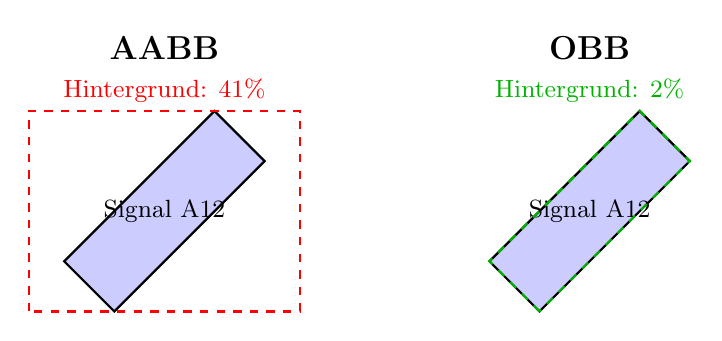
\begin{tikzpicture}[scale=0.9]
    % LEFT: AABB
    \begin{scope}
        \node[above, font=\large\bfseries] at (2, 3.5) {AABB};
        
        % Rotated text at 45 degrees
        \begin{scope}[rotate around={45:(2,1.5)}]
            \draw[thick, fill=blue!20] (0.5,1) rectangle (3.5,2);
            \node[font=\small] at (2,1.5) {Signal A12};
        \end{scope}
        
        % AABB box (red, axis-aligned)
        \draw[thick, red, dashed] (0.086,0.086) rectangle (3.914,2.914);
        
        % Annotations
        \node[below, red, font=\small] at (2, 3.5) {Hintergrund: 41\%};
    \end{scope}
    
    % RIGHT: OBB
    \begin{scope}[xshift=6cm]
        \node[above, font=\large\bfseries] at (2, 3.5) {OBB};
        
        % Rotated text at 45 degrees
        \begin{scope}[rotate around={45:(2,1.5)}]
            \draw[thick, fill=blue!20] (0.5,1) rectangle (3.5,2);
            \node[font=\small] at (2,1.5) {Signal A12};
        \end{scope}
        
        % OBB box (green, rotated with object)
        \begin{scope}[rotate around={45:(2,1.5)}]
            \draw[thick, green!70!black, dashed] (0.5,1) rectangle (3.5,2);
        \end{scope}
        
        % Annotations
        \node[below, green!70!black, font=\small] at (2, 3.5) {Hintergrund: 2\%};
    \end{scope}
\end{tikzpicture}
\caption{AABB vs OBB Vergleich bei rotiertem Textlabel.}
\label{fig:aabb_obb_comparison}
\end{figure}

Dieser hohe Hintergrundanteil hat zwei wesentliche Konsequenzen für die Objekterkennung: Erstens verschlechtert sich das Signal-Rausch-Verhältnis der Eingabedaten für nachgelagerte Verarbeitungsschritte wie OCR\cite{Ma2018ArbitraryOrientedST}. Zweitens steigt die Wahrscheinlichkeit falscher Detektionen, da irrelevante Bildelemente innerhalb der Bounding Box liegen\cite{Ding2019_LearningRoI}.

\subsubsection{Non-Maximum Suppression bei dichten Objektgruppen}

Ein weiteres Problem ergibt sich bei der Nachbearbeitung von Detektionen mittels Non-Maximum Suppression (NMS)\cite{Ren2015_FasterRCNN}. NMS eliminiert redundante Detektionen durch Unterdrückung überlappender Boxen basierend auf ihrer Intersection over Union (IoU):

\begin{equation}
\text{IoU}(B_1, B_2) = \frac{\text{Area}(B_1 \cap B_2)}{\text{Area}(B_1 \cup B_2)}
\end{equation}

Bei dicht platzierten rotierten Objekten führen AABB zu hohen IoU-Werten, obwohl die Objekte selbst nicht überlappen\cite{Ding2019_LearningRoI}. Dies resultiert in fälschlicher Unterdrückung korrekter Detektionen. Abbildung \ref{fig:nms_problem} demonstriert dieses Fehlverhalten anhand zweier nahe beieinanderliegender Textlabels. Die beiden Textobjekte sind um 30° bzw. -30° rotiert und überlappen sich nicht. Ihre achsenparallelen Bounding Boxes hingegen weisen eine signifikante Überlappung mit IoU = 0.42 auf. Bei einem typischen NMS-Schwellenwert von $\tau = 0.4$\cite{Lin2017_FocalLoss} würde eine der beiden korrekten Detektionen fälschlicherweise unterdrückt. Im Gegensatz dazu berechnet sich die IoU zwischen den orientierten Bounding Boxes korrekt zu 0.0, da die Objekte tatsächlich nicht überlappen.

\begin{figure}[H]
\centering
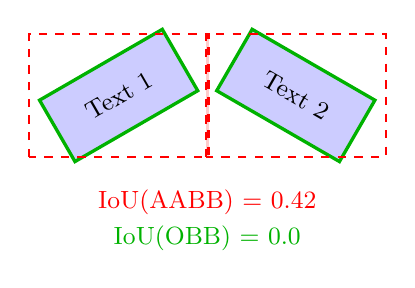
\begin{tikzpicture}[scale=0.9]
    % Two rotated text boxes close together

    % --- Text 1 (30° rotation) ---
    \begin{scope}[rotate around={30:(1.5,2)}]
        \draw[very thick, green!70!black, fill=blue!20] (0.5,1.5) rectangle (2.5,2.5);
        \node[font=\small, rotate=30] at (1.5,2) {Text 1};
    \end{scope}

    % --- Text 2 (-30° rotation) ---
    \begin{scope}[rotate around={-30:(4,2)}]
        \draw[very thick, green!70!black, fill=blue!20] (3,1.5) rectangle (5,2.5);
        \node[font=\small, rotate=-30] at (4,2) {Text 2};
    \end{scope}

    % --- AABBs (red and dashed) ---
    % AABB for Text 1
    \draw[thick, red, dashed] (0.232,1.134) rectangle (2.768,2.866);

    % AABB for Text 2
    \draw[thick, red, dashed] (2.732,1.134) rectangle (5.268,2.866);

    % Overlap region (AABB overlap)
    \fill[red, opacity=0.2] (2.732,1.134) rectangle (2.768,2.866);

    % Annotation
    \node[below, red, font=\small] at (2.75, 0.8) {IoU(AABB) = 0.42};
    \node[below, green!70!black, font=\small] at (2.75, 0.3) {IoU(OBB) = 0.0};
\end{tikzpicture}
\caption{NMS-Problem bei dicht platzierten rotierten Objekten.}
\label{fig:nms_problem}
\end{figure}

\subsection{Oriented Bounding Boxes als Lösung}

Oriented Bounding Boxes erweitern die AABB-Repräsentation um einen zusätzlichen Freiheitsgrad: den Rotationswinkel $\theta$. Eine OBB wird durch fünf Parameter definiert:

\begin{equation}
\text{OBB} = (c_x, c_y, w, h, \theta)
\end{equation}

wobei $(c_x, c_y)$ das Zentrum, $w$ und $h$ die Dimensionen entlang der lokalen Achsen und $\theta \in [-90^\circ, 90^\circ)$ den Rotationswinkel relativ zur horizontalen Bildachse beschreiben. Diese Repräsentation ermöglicht eine eng anliegende Umhüllung rotierter Objekte und reduziert den Hintergrundanteil auf das geometrische Minimum.

\subsubsection{Vorteile für rotierte Objekte}

Die präzisere geometrische Modellierung durch OBB bietet mehrere Vorteile. Bei perfekter Ausrichtung der OBB mit dem Objekt minimiert sich der Hintergrundanteil, während AABB bei starker Rotation erhebliche Hintergrundbereiche umschließen. Die IoU zwischen OBB reflektiert die tatsächliche Objektüberlappung, wodurch Fehlunterdrückungen bei NMS vermieden werden. Dies ist besonders wichtig bei dicht gruppierten Objekten, wo AABB fälschlicherweise hohe Überlappungen anzeigen würden. Zudem kodiert der Parameter $\theta$ explizit die Objektorientierung, was für nachgelagerte Prozesse wie orientierungsabhängige OCR wertvoll ist. Für die Domäne der Gleisplan-Analyse sind diese Eigenschaften besonders relevant, da Symbole entlang der Gleisachsen in beliebigen Winkeln angeordnet sind und oft dicht gruppiert auftreten.

\subsection{Herausforderungen bei der Verwendung von OBB}

Trotz der geometrischen Vorteile bringen OBB zusätzliche Komplexität in die Detektionspipeline, die sich auf Training, Inferenz und Nachbearbeitung auswirkt. Abbildung \ref{fig:obb_challenges} fasst die drei Hauptherausforderungen zusammen: erhöhte Berechnungskomplexität bei der IoU-Berechnung, die Periodizität des Rotationswinkels, die zu Trainingsinstabilität führt, und der erhöhte Trainingsaufwand gegenüber AABB-Modellen.

\begin{figure}[H]
\centering
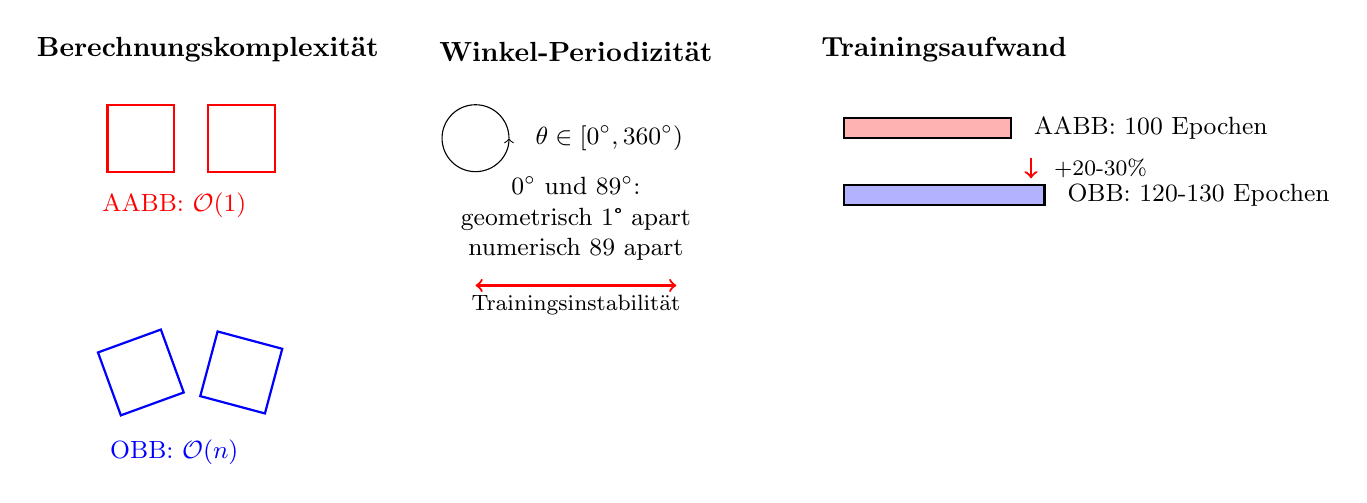
\begin{tikzpicture}[scale=0.85, every node/.style={font=\small}]
    % Challenge 1: Computational Complexity
    \begin{scope}
        \node[above, font=\bfseries] at (2, 3.5) {Berechnungskomplexität};
        
        % AABB: Simple rectangles
        \draw[thick, red] (0.5, 2) rectangle (1.5, 3);
        \draw[thick, red] (2, 2) rectangle (3, 3);
        \node at (1.5, 1.5) {\textcolor{red}{AABB: $\mathcal{O}(1)$}};
        
        % OBB: Rotated rectangles with intersection
        \begin{scope}[shift={(0,-1.5)}]
            \begin{scope}[rotate around={20:(1,0.5)}]
                \draw[thick, blue] (0.5, 0) rectangle (1.5, 1);
            \end{scope}
            \begin{scope}[rotate around={-15:(2.5,0.5)}]
                \draw[thick, blue] (2, 0) rectangle (3, 1);
            \end{scope}
            \node at (1.5, -0.7) {\textcolor{blue}{OBB: $\mathcal{O}(n)$}};
        \end{scope}
    \end{scope}
    
    % Challenge 2: Angle Periodicity
    \begin{scope}[xshift=5.5cm]
        \node[above, font=\bfseries] at (2, 3.5) {Winkel-Periodizität};
        
        % Angle representation
        \draw[->] (1, 2.5) arc (0:360:0.5);
        \node at (2.5, 2.5) {$\theta \in [0^\circ, 360^\circ)$};
        
        % Problem illustration
        \node[align=center] at (2, 1.3) {$0^\circ$ und $89^\circ$:\\geometrisch 1° apart\\numerisch 89 apart};
        
        \draw[thick, red, <->] (0.5, 0.3) -- (3.5, 0.3);
        \node[below, font=\footnotesize] at (2, 0.3) {Trainingsinstabilität};
    \end{scope}
    
    % Challenge 3: Training Overhead
    \begin{scope}[xshift=11cm]
        \node[above, font=\bfseries] at (2, 3.5) {Trainingsaufwand};
        
        % Training progress bars
        \draw[thick, fill=red!30] (0.5, 2.5) rectangle (3, 2.8);
        \node[right] at (3.2, 2.65) {AABB: 100 Epochen};
        
        \draw[thick, fill=blue!30] (0.5, 1.5) rectangle (3.5, 1.8);
        \node[right] at (3.7, 1.65) {OBB: 120-130 Epochen};
        
        % Arrow indicating increase
        \draw[thick, red, ->] (3.3, 2.2) -- (3.3, 1.9);
        \node[right, font=\footnotesize] at (3.5, 2.05) {+20-30\%};
    \end{scope}
\end{tikzpicture}
\caption{Hauptherausforderungen bei OBB-Verwendung.}
\label{fig:obb_challenges}
\end{figure}

\subsubsection{Erhöhte Berechnungskomplexität}

Die Berechnung der Intersection over Union zwischen zwei OBB ist algorithmisch aufwendiger als bei AABB. Während die AABB-IoU durch einfache Min-Max-Operationen in konstanter Zeit $\mathcal{O}(1)$ berechnet werden kann, erfordert die OBB-IoU die Lösung eines Polygon-Clipping-Problems\cite{Zhou2017EastAE}:

\begin{equation}
\text{IoU}_{\text{OBB}}(B_1, B_2) = \frac{\text{Area}(P_1 \cap P_2)}{\text{Area}(P_1 \cup P_2)}
\end{equation}

wobei $P_1$ und $P_2$ die als Vierecke repräsentierten OBB sind. Die Schnittpunktberechnung zwischen den Kantensegmenten skaliert mit $\mathcal{O}(n^2)$ für $n$-Ecke, was in der Praxis zu einem Faktor 3-5 langsameren NMS-Durchläufen führt\cite{Xie2021OrientedRD}.

\subsubsection{Winkel-Periodizität und Trainingsinstabilität}

Der Rotationswinkel $\theta$ weist eine zyklische Periodizität auf: Eine Rotation um 180° (bzw. bei symmetrischen Objekten um 90°) resultiert in einer geometrisch identischen Bounding Box\cite{Yang2021RSDETR,Zhao2023ABFL}. Dies führt zu Ambiguitäten in der Netzwerk-Ausgabe. Betrachtet man beispielsweise zwei Vorhersagen $\theta_1 = 0^\circ$ und $\theta_2 = 89^\circ$ für dasselbe Objekt, so sind diese geometrisch nur 1° voneinander entfernt, numerisch jedoch 89 Einheiten. Standard-Regressionsverluste (z.B. Smooth L1) behandeln diese Diskrepanz linear, was zu instabilen Gradienten führt.


\subsubsection{Erhöhter Trainingsaufwand}

Die zusätzliche Parameterregression für $\theta$ erhöht die Komplexität des Lernproblems. Empirische Studien zeigen, dass OBB-Modelle typischerweise 20-30\% mehr Trainingsepochen benötigen als vergleichbare AABB-Modelle, um ähnliche Konvergenzniveaus zu erreichen\cite{Xie2021OrientedRD}. Dies resultiert aus der Notwendigkeit, sowohl die präzise Lokalisierung als auch die korrekte Orientierungsprädiktion zu erlernen.

\subsection{YOLOv8-OBB Architektur}

Die in Kapitel 5 motivierte Wahl von YOLOv8 für die Symbolerkennung basiert auf dessen spezialisierter OBB-Variante. YOLOv8-OBB erweitert die Standard-Architektur um die Regression des Rotationsparameters $\theta$, während die grundlegende Netzwerkstruktur aus Backbone, Neck und Detection Heads erhalten bleibt\cite{yolov8_ultralytics}. Die schematische Architektur ist in Abbildung \ref{fig:yolov8_architecture} dargestellt und zeigt den Informationsfluss vom Eingabebild über die Feature-Extraktion bis zu den finalen OBB-Vorhersagen. Der Backbone extrahiert hierarchische Merkmale auf fünf Auflösungsstufen, das Neck fusioniert diese über Skalen hinweg, und die drei spezialisierten Detection Heads produzieren Vorhersagen für kleine, mittlere und große Objekte.

\begin{figure}[H]
\centering
\hspace*{1.5cm} 
\begin{tikzpicture}[
    scale=0.9,
    node distance=1.2cm and 0.5cm,
    module/.style={
        rectangle, 
        draw, 
        minimum width=3.2cm, 
        minimum height=1cm, 
        align=center, 
        fill=blue!10,
        font=\small
    },
    arrow/.style={->, >=stealth, thick, rounded corners}
]

    % 1. Input
    \node[module, fill=gray!20] (input) {Input\\$1024 \times 1024 \times 3$};
    
    % 2. Backbone
    \node[module, below=of input, fill=blue!20] (backbone) {CSPNet Backbone\\(C2f Modules)};
    
    % 3. Multi-scale features
    \node[module, below=of backbone, fill=green!20, minimum width=8cm] (features) {Multi-Scale Features\\(P3, P4, P5)};
    
    % 4. Neck
    \node[module, below=of features, fill=orange!20] (neck) {PANet Neck\\(FPN + PAN)};
    
    % 5. Detection heads
    \node[module, below=1.5cm of neck, fill=red!20, minimum width=2.8cm] (head2) {Head P4\\(Medium)};
    \node[module, left=0.2cm of head2, fill=red!20, minimum width=2.8cm] (head1) {Head P3\\(Small)};
    \node[module, right=0.2cm of head2, fill=red!20, minimum width=2.8cm] (head3) {Head P5\\(Large)};
    
    % 6. Outputs
    \node[module, below=1.2cm of head2, fill=purple!20, minimum width=8cm] (output) {OBB Predictions\\$(c_x, c_y, w, h, \theta, \text{cls})$};
    
    % Arrows
    \draw[arrow] (input) -- (backbone);
    \draw[arrow] (backbone) -- (features);
    \draw[arrow] (features) -- (neck);
    
    \draw[arrow] (neck.south) -- (head2.north); 
    \draw[arrow] (neck.south) -| (head1.north); 
    \draw[arrow] (neck.south) -| (head3.north); 
    
    \draw[arrow] (head2.south) -- (output.north);
    \draw[arrow] (head1.south) -- (head1.south |- output.north); 
    \draw[arrow] (head3.south) -- (head3.south |- output.north); 
    
    % Annotations
    \node[right=0.8cm of backbone, font=\footnotesize, align=left] {
        \textbf{Feature Extraction:}\\
        5 Resolution Levels
    };
    
    \node[right=0.8cm of neck, font=\footnotesize, align=left] {
        \textbf{Feature Fusion:}\\
        Top-Down + Bottom-Up
    };
    
    \node[right=0.2cm of head3, font=\footnotesize, align=left, text width=3.5cm] {
        \textbf{Decoupled Heads:}\\
        Separate Classification\\
        \& Regression
    };

\end{tikzpicture}
\caption{YOLOv8-OBB Architektur.}
\label{fig:yolov8_architecture}
\end{figure}

\subsubsection{Netzwerkkomponenten}

Die Architektur gliedert sich in drei funktionale Blöcke. Der Backbone extrahiert hierarchische Merkmale aus den Eingabebildern und verwendet eine auf CSPNet basierende Architektur mit Cross Stage Partial Connections\cite{Wang2020_CSPNet}. Die sogenannten C2f-Module (CSP Bottleneck with 2 Convolutions, faster) ersetzen die C3-Module früherer Versionen und bieten eine effizientere Gradientenfluss-Charakteristik bei gleichzeitiger Reduktion der Parameteranzahl. Das Neck-Modul fusioniert Merkmale unterschiedlicher Auflösungsstufen durch eine Kombination aus Top-Down- und Bottom-Up-Pfaden. Die Path Aggregation Network (PANet) Architektur\cite{Liu2018_PANet} ermöglicht eine effektive Informationspropagation zwischen den Skalen, was für die Detektion sowohl kleiner als auch großer Objekte essentiell ist. YOLOv8 folgt einem Anchor-Free-Ansatz\cite{Tian2019FCOS}, bei dem Objektzentren direkt vorhergesagt werden, anstatt vordefinierte Anker-Boxen zu verwenden. Die Heads sind dezentralisiert (decoupled): Separate Zweige regredieren die Lokalisierung (inklusive $\theta$) und die Klassifikation. Diese Entkopplung verbessert die Konvergenz, da die beiden Aufgaben unterschiedliche Repräsentationen erfordern\cite{Ge2021_YOLOX}.

\subsubsection{Verlustfunktion und Training}

Das Training von YOLOv8-OBB optimiert eine kombinierte Verlustfunktion, die drei Komponenten umfasst:

\begin{equation}
\mathcal{L}_{\text{total}} = \lambda_{\text{box}} \mathcal{L}_{\text{box}} + \lambda_{\text{cls}} \mathcal{L}_{\text{cls}} + \lambda_{\text{dfl}} \mathcal{L}_{\text{dfl}}
\end{equation}

Die Box-Loss $\mathcal{L}_{\text{box}}$ quantifiziert die Lokalisierungsgenauigkeit der vorhergesagten OBB gegenüber der Ground Truth. Die Classification-Loss $\mathcal{L}_{\text{cls}}$ verwendet Binary Cross-Entropy für die Klassenzuordnung\cite{Lin2017_FocalLoss}. Die Distribution Focal Loss (DFL)\cite{Li2020GeneralizedFocal} verbessert die Bounding-Box-Regression durch Modellierung der Koordinaten als Verteilungen anstelle von Punktschätzungen.

Die konkreten Trainingsparameter und -ergebnisse für den im Rahmen dieser Arbeit trainierten Detektor werden in Kapitel 6 detailliert dokumentiert. Die Auswahl von YOLOv8-OBB in Kapitel 5 basiert auf der Kombination aus Echtzeitfähigkeit, Rotationsinvarianz und dem Anchor-Free-Design, welches die Adaption an domänenspezifische Symbolklassen erleichtert.

\subsection{Relevanz für Gleisplan-Analyse}

Die beschriebenen OBB-Eigenschaften sind besonders relevant für die automatisierte Analyse von Gleisplänen. Technische Zeichnungen dieses Typs weisen drei charakteristische Merkmale auf, die den Einsatz orientierter Bounding Boxes notwendig machen. Symbole folgen der Topologie der Gleisachsen und können daher in jedem Winkel $\theta \in [0^\circ, 360^\circ)$ vorliegen. In Bahnhöfen und Weichenstraßen treten Symbole räumlich konzentriert auf, wobei AABB-basierte NMS zu Fehlunterdrückungen führen würde. Die vom OBB-Detektor gelieferte Rotation $\theta$ ist für nachgelagerte Prozesse wie die orientierungsabhängige OCR (vgl. Kapitel 6.3) essentiell, da Textlabels entsprechend ihrer Ausrichtung verarbeitet werden müssen.

Die in Kapitel 4 definierten funktionalen Anforderungen an die Symbolerkennung erfordern daher zwingend den Einsatz rotationsinvarianter Detektionsverfahren. Die in Kapitel 6 beschriebene Implementierung nutzt YOLOv8-OBB mit Standard-Konfiguration für die Detektion von 13 domänenspezifischen Symbolklassen (vgl. Tabelle \ref{tab:symbole} in Kapitel 4).

\section{Optical Character Recognition (OCR)}
\label{sec:ocr}

Die optische Zeichenerkennung bildet das verbindende Element zwischen der visuellen Symbolerkennung und der semantischen Interpretation von Gleisplänen. Während die in Abschnitt \ref{sec:objekterkennung} beschriebene Objekterkennung Symbole lokalisiert und klassifiziert, liefert sie zunächst keine Information über die zugehörigen Textinhalte. Erst durch die zuverlässige Extraktion von Signalbezeichnungen (z.\,B. \enquote{AS102}), Kilometerangaben (z.\,B. \enquote{18.1606}) und Balisen-Kennungen (z.\,B. \enquote{1234}) erhalten die erkannten Symbole ihre vollständige technische Bedeutung.

Dieser Abschnitt behandelt zunächst die allgemeinen Grundlagen der optischen Zeichenerkennung, bevor die spezifischen Herausforderungen technischer Zeichnungen und die für Gleispläne relevanten Lösungsansätze dargelegt werden. Die Progression folgt dabei dem Muster der vorangegangenen Abschnitte: vom allgemeinen Prinzip über moderne Architekturen bis zur domänenspezifischen Anwendung.

\subsection{Grundlagen und Entwicklung der OCR-Technologie}
\label{subsec:ocr_grundlagen}

Die optische Zeichenerkennung bezeichnet die automatisierte Umwandlung von Bildern, die Text enthalten, in maschinenlesbaren Text. Diese Aufgabe lässt sich konzeptionell in eine Verarbeitungskette unterteilen, die in Abbildung \ref{fig:ocr_pipeline_konzept} dargestellt ist.

\begin{figure}[h]
\centering
\begin{tikzpicture}[
    % Größerer vertikaler Abstand (2.5cm) für die Labels dazwischen
    node distance=2.5cm and 1.0cm,
    box/.style={
        rectangle, 
        draw, 
        thick, 
        minimum width=3.2cm, % Etwas breiter für besseren Textumbruch
        minimum height=1cm, 
        align=center, 
        font=\small, 
        rounded corners=2pt
    },
    arrow/.style={->, >=stealth, thick, rounded corners},
    annotation/.style={font=\scriptsize, align=center, text=gray!40!black}
]

    % --- ZEILE 1 (Nach Rechts) ---
    
    % 1. Input
    \node[box, fill=blue!10] (input) {Eingabebild\\(Dokument/Scan)};
    
    % 2. Vorverarbeitung
    \node[box, right=of input, fill=yellow!20] (preproc) {Vorverarbeitung\\(Binarisierung)};
    \node[annotation, below=0.1cm of preproc] {Kontrast,\\Rauschen};
    
    % 3. Textdetektion
    \node[box, right=of preproc, fill=orange!20] (detect) {Textdetektion\\(Lokalisierung)};
    \node[annotation, below=0.1cm of detect] {Bounding\\Boxes};

    
    % --- ZEILE 2 (Nach Links, unter der ersten Zeile) ---
    
    % 4. Zeichenerkennung (Unter Detektion)
    \node[box, below=of detect, fill=green!20] (recog) {Zeichenerkennung\\(Recognition)};
    \node[annotation, below=0.1cm of recog] {CNN/LSTM\\Decoder};
    
    % 5. Nachverarbeitung (Links von Erkennung)
    \node[box, left=of recog, fill=purple!20] (post) {Nachverarbeitung\\(Validierung)};
    \node[annotation, below=0.1cm of post] {Regex,\\Korrektur};
    
    % 6. Ausgabe (Links von Post)
    \node[box, left=of post, fill=gray!10] (output) {Ausgabetext\\(String)};
    

    % --- PFEILE ---
    \draw[arrow] (input) -- (preproc);
    \draw[arrow] (preproc) -- (detect);
    
    % Der Pfeil von Zeile 1 zu Zeile 2 (Rechts außen runter)
    \draw[arrow] (detect.south) -- (recog.north);
    
    % Pfeile zurück nach links
    \draw[arrow] (recog) -- (post);
    \draw[arrow] (post) -- (output);

\end{tikzpicture}
\caption{Konzeptionelle OCR-Pipeline (Zweizeilige Darstellung)}
\label{fig:ocr_pipeline_konzept}
\end{figure}
Die \textbf{Vorverarbeitung} bereitet das Eingabebild für die nachfolgenden Schritte auf. Typische Operationen umfassen Kontrastverbesserung, Rauschunterdrückung und Binarisierung (Umwandlung in Schwarz-Weiß). Bei technischen Zeichnungen ist zusätzlich die Entfernung störender Linienelemente relevant \cite{Tombre}.

Die \textbf{Textdetektion} lokalisiert Bereiche im Bild, die Text enthalten. Moderne Verfahren verwenden neuronale Netze zur Segmentierung von Textregionen, wobei die Ausgabe typischerweise als Bounding Boxes oder Polygone erfolgt \cite{liao2019realtimescenetextdetection}.

Die \textbf{Zeichenerkennung} wandelt die lokalisierten Bildausschnitte in Zeichenfolgen um. Dies ist die eigentliche \enquote{Erkennung} im engeren Sinne und bildet den rechenintensivsten Schritt der Pipeline.

Die \textbf{Nachverarbeitung} validiert und korrigiert die erkannten Texte. Für domänenspezifische Anwendungen wie Gleispläne können hier Musterprüfungen (Regular Expressions) und Plausibilitätskontrollen integriert werden.

\subsubsection{Historische Entwicklung}

Die Entwicklung der OCR-Technologie lässt sich in drei Phasen unterteilen, die in Tabelle \ref{tab:ocr_evolution} zusammengefasst sind.

\begin{table}[H]
\centering
\renewcommand{\arraystretch}{1.3}
\begin{tabular}{|p{2.5cm}|p{3cm}|p{4cm}|p{4cm}|}
\hline
\textbf{Phase} & \textbf{Zeitraum} & \textbf{Methodik} & \textbf{Limitierungen} \\
\hline
Regelbasiert & 1950--1980 & Template Matching, Merkmalsdeskriptoren & Nur monospace-Schriften, keine Variabilität \\
\hline
Statistisch & 1980--2010 & Hidden Markov Models (HMM), SVM mit HOG-Features & Manuelles Feature-Engineering, begrenzte Robustheit \\
\hline
Deep Learning & 2010--heute & CNN + RNN, Transformer, End-to-End-Training & Hoher Datenbedarf, Rechenaufwand \\
\hline
\end{tabular}
\caption{Evolution der OCR-Technologie über drei methodische Phasen\cite{Mori1999}}
\label{tab:ocr_evolution}
\end{table}

Die erste Generation basierte auf expliziten Mustervergleichen: Für jedes zu erkennende Zeichen wurde ein Template definiert, das pixelweise mit dem Eingabebild verglichen wurde \cite{Mori1999}. Diese Ansätze funktionierten nur bei exakt passenden Schriftarten und -größen.

Die zweite Generation führte statistische Modelle ein. Hidden Markov Models (HMM) modellierten die sequenzielle Struktur von Text, während Support Vector Machines (SVM) auf manuell konstruierten Merkmalen (z.\,B. Histogram of Oriented Gradients) operierten \cite{Smith2007}. Diese Verfahren ermöglichten erstmals Robustheit gegenüber moderaten Variationen, erforderten jedoch aufwendiges Feature-Engineering.

Die dritte Generation nutzt Deep Learning für End-to-End-Erkennung. Convolutional Neural Networks (CNN) extrahieren visuelle Merkmale automatisch aus Trainingsbeispielen, während Recurrent Neural Networks (RNN) die sequenzielle Abhängigkeit zwischen Zeichen modellieren \cite{Shi2017_CRNN}. Diese Kombination ermöglicht die Erkennung beliebiger Schriftarten und -stile ohne manuelle Merkmalsdefiniton.

\subsection{Architekturen moderner OCR-Systeme}
\label{subsec:ocr_architekturen}

Moderne OCR-Systeme basieren auf zwei dominierenden Architekturparadigmen: der CRNN-Architektur (Convolutional Recurrent Neural Network) und Transformer-basierten Ansätzen. Beide werden im Folgenden erläutert.

\subsubsection{CRNN-Architektur}

Die CRNN-Architektur, eingeführt von Shi et al. \cite{Shi2017_CRNN}, kombiniert drei Komponenten zu einem End-to-End-trainierbaren System (Abbildung \ref{fig:crnn_architecture}).

\begin{figure}[H]
\centering
\begin{tikzpicture}[
    scale=0.8,
    node distance=1.0cm and 0.8cm,
    layer/.style={rectangle, draw, thick, minimum width=2.2cm, minimum height=0.9cm, align=center, font=\small},
    arrow/.style={->, >=stealth, thick}
]
    % Input
    \node[layer, fill=gray!20] (input) {Bildausschnitt\\$W \times H \times 1$};
    
    % CNN Layers
    \node[layer, below=of input, fill=blue!20] (cnn1) {Conv + Pool\\$\times 4$};
    \node[layer, below=of cnn1, fill=blue!30] (cnn2) {Feature Maps\\$\frac{W}{4} \times 1 \times 512$};
    
    % Reshape
    \node[layer, below=of cnn2, fill=yellow!30] (reshape) {Reshape\\Sequenz von $T$ Vektoren};
    
    % BiLSTM
    \node[layer, below=of reshape, fill=orange!30] (lstm) {BiLSTM\\2 Schichten, 256 Hidden};
    
    % CTC
    \node[layer, below=of lstm, fill=green!30] (ctc) {CTC-Decoder\\Alignment + Deduplizierung};
    
    % Output
    \node[layer, below=of ctc, fill=purple!20] (output) {Ausgabetext\\z.\,B. \enquote{AS102}};
    
    % Arrows
    \draw[arrow] (input) -- (cnn1);
    \draw[arrow] (cnn1) -- (cnn2);
    \draw[arrow] (cnn2) -- (reshape);
    \draw[arrow] (reshape) -- (lstm);
    \draw[arrow] (lstm) -- (ctc);
    \draw[arrow] (ctc) -- (output);
    
    % Side labels
    \node[right=0.5cm of cnn1, font=\scriptsize, align=left] {Visuelle\\Merkmale};
    \node[right=0.5cm of lstm, font=\scriptsize, align=left] {Sequenzielle\\Abhängigkeiten};
    \node[right=0.5cm of ctc, font=\scriptsize, align=left] {Variable\\Längen};
    
    % Component brackets
    \draw[decorate, decoration={brace, amplitude=5pt}, thick] 
        ([xshift=-0.3cm]cnn1.north west) -- ([xshift=-0.3cm]cnn2.south west) 
        node[midway, left=8pt, font=\small\bfseries] {CNN};
    \draw[decorate, decoration={brace, amplitude=5pt}, thick] 
        ([xshift=-0.3cm]lstm.north west) -- ([xshift=-0.3cm]lstm.south west) 
        node[midway, left=8pt, font=\small\bfseries] {RNN};
    \draw[decorate, decoration={brace, amplitude=5pt}, thick] 
        ([xshift=-0.3cm]ctc.north west) -- ([xshift=-0.3cm]ctc.south west) 
        node[midway, left=8pt, font=\small\bfseries] {CTC};
\end{tikzpicture}
\caption{CRNN-Architektur}
\label{fig:crnn_architecture}
\end{figure}

\textbf{CNN-Komponente (Feature Extraction):} Ein Convolutional Neural Network extrahiert visuelle Merkmale aus dem Eingabebild. Durch sukzessive Faltungs- und Pooling-Operationen wird das Bild auf eine Sequenz von Merkmalsvektoren reduziert. Ein Bildausschnitt der Größe $W \times H$ wird typischerweise auf $T = W/4$ Zeitschritte mit je 512 Merkmalskanälen komprimiert\cite{Shi2017_CRNN}.

\textbf{RNN-Komponente (Sequence Modeling):} Ein bidirektionales LSTM (Long Short-Term Memory) \cite{Hochreiter1997_LSTM} verarbeitet die Merkmalssequenz und modelliert kontextuelle Abhängigkeiten zwischen benachbarten Zeichen. Die Bidirektionalität ermöglicht die Berücksichtigung sowohl vergangener als auch zukünftiger Kontextinformation.

\textbf{CTC-Decoder (Transcription):} Die Connectionist Temporal Classification (CTC) \cite{Graves2006_CTC} löst das Problem variabler Ausgabelängen. Da die Anzahl der CNN-Ausgabespalten nicht mit der Anzahl der Textzeichen übereinstimmt, führt CTC ein \enquote{Blank}-Symbol ein und definiert eine Verlustfunktion, die alle möglichen Alignments zwischen Eingabe und Ausgabe marginalisiert:

\begin{equation}
P(y \mid x) = \sum_{\pi \in \mathcal{B}^{-1}(y)} \prod_{t=1}^{T} P(\pi_t \mid x)
\label{eq:ctc_loss}
\end{equation}

wobei $y$ die Zielsequenz, $x$ die Eingabe, $\mathcal{B}^{-1}(y)$ die Menge aller Pfade bezeichnet, die nach Entfernung von Blanks und Deduplizierung $y$ ergeben, und $P(\pi_t \mid x)$ die Wahrscheinlichkeit des Symbols $\pi_t$ zum Zeitpunkt $t$ ist.

Für Maschinenbau-Ingenieure lässt sich die CTC-Funktionsweise anschaulich erklären: Das Netz gibt für jeden Zeitschritt (jede Spalte des Bildes) eine Wahrscheinlichkeitsverteilung über alle möglichen Zeichen aus. Die Ausgabe \enquote{A--S-11-0-2} (wobei \enquote{-} das Blank-Symbol bezeichnet) wird durch Entfernung der Blanks und Zusammenfassung aufeinanderfolgender identischer Zeichen zu \enquote{AS102} dekodiert.

\subsubsection{Transformer-basierte OCR}

Neuere Ansätze ersetzen die RNN-Komponente durch Transformer-Architekturen \cite{Vaswani2017_Attention}. Der TrOCR-Ansatz \cite{li2022trocrtransformerbasedopticalcharacter} verwendet einen Vision Transformer (ViT) als Encoder und einen Text Transformer als Decoder. Vision Transformer ist ein Transformer Modell, das Bilder als Sequenz von Patches verarbeitet\cite{Dosovitskiy2021_ViT} Der zentrale Mechanismus ist die Self-Attention:

\begin{equation}
\text{Attention}(Q, K, V) = \text{softmax}\left(\frac{QK^T}{\sqrt{d_k}}\right) V
\label{eq:attention}
\end{equation}

wobei $Q$ (Query), $K$ (Key) und $V$ (Value) lineare Projektionen der Eingabe sind und $d_k$ die Dimensionalität der Keys bezeichnet. Die Division durch $\sqrt{d_k}$ stabilisiert die Gradienten.

Transformer-basierte Ansätze bieten Vorteile bei langen Sequenzen und ermöglichen effizientere Parallelisierung während des Trainings. Für kurze Texte wie Signalbezeichnungen (typischerweise 3--8 Zeichen) sind die Vorteile jedoch marginal, weshalb CRNN-basierte Systeme wie PaddleOCR in der Praxis häufig bevorzugt werden.

\subsubsection{Vergleich der Architekturen}

Tabelle \ref{tab:ocr_arch_comparison} fasst die wesentlichen Unterschiede zwischen CRNN und Transformer-basierten Ansätzen zusammen.
\begin{table}[H]
\centering
\renewcommand{\arraystretch}{1.3}
\begin{tabular}{|p{3.5cm}|p{5cm}|p{5cm}|}
\hline
\textbf{Kriterium} & \textbf{CRNN (z.\,B. PaddleOCR)} & \textbf{Transformer (z.\,B. TrOCR)} \\
\hline
Genauigkeit (kurze Texte) & >95\% \cite{du2020ppocrpracticalultralightweight} & >95\% \cite{li2022trocrtransformerbasedopticalcharacter} \\
\hline
Inferenzzeit (CPU) & 8--15 ms/Bild \cite{du2020ppocrpracticalultralightweight} & 50--150 ms/Bild\footnotemark \\
\hline
Modellgröße & 8--12 MB \cite{du2020ppocrpracticalultralightweight} & 300--500 MB \cite{li2022trocrtransformerbasedopticalcharacter} \\
\hline
Trainingsdatenbedarf & Moderat (10k--100k Samples) & Hoch (>1M Samples für Pretraining) \cite{li2022trocrtransformerbasedopticalcharacter} \\
\hline
\end{tabular}
\caption{Vergleich von CRNN- und Transformer-basierten OCR-Architekturen}
\label{tab:ocr_arch_comparison}
\end{table}
\footnotetext{Transformer-basierte Modelle erfordern aufgrund des quadratischen 
Attention-Mechanismus höhere Inferenzzeiten \cite{Vaswani2017_Attention}.}

\subsection{OCR-Systeme im praktischen Einsatz}
\label{subsec:ocr_systeme}

Für die praktische Anwendung stehen mehrere etablierte OCR-Frameworks zur Verfügung, die unterschiedliche Stärken aufweisen.

\subsubsection{Tesseract}

Tesseract \cite{Smith2007} ist eine Open-Source-Engine, die ursprünglich von Hewlett-Packard entwickelt und später von Google weiterentwickelt wurde. Seit Version 4.0 verwendet Tesseract ein LSTM-basiertes Erkennungsmodell. Die Konfiguration erfolgt über Page Segmentation Modes (PSM), die das erwartete Dokumentlayout spezifizieren:

\begin{itemize}
    \item \textbf{PSM 7}: Einzelne Textzeile -- optimal für isolierte Beschriftungen
    \item \textbf{PSM 8}: Einzelnes Wort -- für kompakte Labels
    \item \textbf{PSM 13}: Raw Line -- für einzelne Textzeilen ohne Layoutsegmentierung, optimal für isolierte Beschriftungen
\end{itemize}

Eine Whitelist-Funktionalität ermöglicht die Einschränkung des Zeichensatzes auf erwartete Zeichen (z.\,B. nur Großbuchstaben und Ziffern für Signalbezeichnungen), was die Erkennungsgenauigkeit in domänenspezifischen Anwendungen erhöht.

\subsubsection{PaddleOCR}

PaddleOCR \cite{du2020ppocrpracticalultralightweight} ist ein vom chinesischen Technologiekonzern Baidu entwickeltes Framework, das eine vollständige Pipeline aus Textdetektion, Winkelklassifikation und Texterkennung bereitstellt. Die PP-OCRv3-Architektur besteht aus drei Komponenten:

\begin{enumerate}
    \item \textbf{DB-Detektor (Differentiable Binarization)}: Lokalisiert Textregionen durch semantische Segmentierung mit differenzierbarer Schwellenwertberechnung \cite{liao2019realtimescenetextdetection}.
    \item \textbf{Winkelklassifikator}: Bestimmt die Orientierung des Textes (0° oder 180°) zur automatischen Korrektur.
    \item \textbf{CRNN-Recognizer}: Erkennt die Zeichenfolge basierend auf der in Abschnitt \ref{subsec:ocr_architekturen} beschriebenen Architektur.
\end{enumerate}

\begin{figure}[H]
\centering
\begin{tikzpicture}[
    scale=0.85,
    node distance=1.5cm,
    box/.style={rectangle, draw, thick, minimum width=3cm, minimum height=1cm, align=center, font=\small, rounded corners=2pt},
    arrow/.style={->, >=stealth, thick}
]
    % Input
    \node[box, fill=gray!20] (input) {Eingabebild};
    
    % Detection
    \node[box, below=of input, fill=blue!20] (detect) {DB-Detektor\\(Texterkennung)};
    
    % Crop
    \node[box, below=of detect, fill=yellow!20] (crop) {ROI-Extraktion\\(Bildausschnitte)};
    
    % Angle
    \node[box, below left=1cm and 0.5cm of crop, fill=orange!20] (angle) {Winkel-\\Klassifikator};
    
    % Recognition
    \node[box, below right=1cm and 0.5cm of crop, fill=green!20] (recog) {CRNN-\\Recognizer};
    
    % Output
    \node[box, below=2.5cm of crop, fill=purple!20] (output) {Erkannte Texte\\+ Positionen};
    
    % Arrows
    \draw[arrow] (input) -- (detect);
    \draw[arrow] (detect) -- (crop);
    \draw[arrow] (crop) -| (angle);
    \draw[arrow] (crop) -| (recog);
    \draw[arrow] (angle) |- (output);
    \draw[arrow] (recog) |- (output);
    
    % Annotations
    \node[right=0.3cm of detect, font=\scriptsize, align=left] {Polygone/Boxes\\für Textregionen};
    \node[left=0.3cm of angle, font=\scriptsize, align=right] {0° oder 180°\\Korrektur};
    \node[right=0.3cm of recog, font=\scriptsize, align=left] {Zeichenfolge\\+ Konfidenz};
\end{tikzpicture}
\caption{PaddleOCR-Pipeline: Dreistufige Architektur mit Detektion, Winkelkorrektur und Erkennung.}
\label{fig:paddleocr_pipeline}
\end{figure}

\subsubsection{Vergleich der OCR-Systeme}

Tabelle \ref{tab:ocr_systems_comparison} vergleicht die für technische Zeichnungen relevanten OCR-Systeme.

\begin{table}[H]
\centering
\small
\renewcommand{\arraystretch}{1.3}
\begin{tabular}{|p{2cm}|p{2.5cm}|p{4.5cm}|p{4.5cm}|}
\hline
\textbf{System} & \textbf{Architektur} & \textbf{Stärken} & \textbf{Schwächen} \\
\hline
Tesseract & LSTM-basiert & Whitelist-Funktion, geringer Ressourcenbedarf & Empfindlich bei Rotation, langsam bei vielen ROIs \\
\hline
PaddleOCR & DB + CRNN & Integrierte Winkelerkennung, schnell, robust & Komplexere Installation, größeres Modell\\
\hline
EasyOCR & CRAFT(Character Region Awareness for Text) + CRNN \cite{baek2019characterregionawarenesstext} & Einfache API, gute Winkeltoleranz & Langsamer, weniger konfigurierbar \\
\hline
TrOCR & Transformer & State-of-the-Art Genauigkeit & Hoher GPU-Bedarf, langsam\\
\hline
\end{tabular}
\caption{Vergleich etablierter OCR-Systeme für technische Anwendungen}
\label{tab:ocr_systems_comparison}
\end{table}

\subsection{Herausforderungen bei technischen Zeichnungen}
\label{subsec:ocr_challenges}

Technische Zeichnungen wie Gleispläne stellen OCR-Systeme vor spezifische Herausforderungen, die über typische Dokumentenscans hinausgehen. Diese Herausforderungen werden in Abbildung \ref{fig:ocr_challenges_fixed_black} visualisiert.

\begin{figure}[H]
\centering
\begin{tikzpicture}[
    % Global settings
    node distance=0.3cm, 
    box/.style={
        rectangle, 
        draw=black,          % <--- ÄNDERUNG: Schwarzer Rahmen
        thick, 
        minimum width=3.6cm, 
        minimum height=4.5cm, 
        align=center, 
        fill=white, 
        rounded corners=3pt
        % <--- ÄNDERUNG: drop shadow entfernt
    },
    title/.style={
        font=\bfseries\small,
        anchor=north,
        yshift=-0.2cm
    },
    footer/.style={
        font=\scriptsize, 
        text=black,          % <--- ÄNDERUNG: Schwarzer Text
        anchor=south,
        yshift=0.2cm
    }
]

    % ==========================================
    % 1. ROTATION
    % ==========================================
    \node[box] (rot) {};
    \node[title] at (rot.north) {Rotation};
    
    % Inhalt vergrößert
    \begin{scope}[shift={(rot.center)}, yshift=0.1cm]
        \node[draw=blue!50!black, fill=blue!10, inner sep=2pt, font=\scriptsize, rotate=15] at (0, 0.9) {AS102};
        \node[draw=blue!50!black, fill=blue!10, inner sep=2pt, font=\scriptsize, rotate=-45] at (-0.7, 0) {BHR01};
        \node[draw=blue!50!black, fill=blue!10, inner sep=2pt, font=\scriptsize, rotate=90] at (0.9, -0.2) {F3};
        \node[draw=blue!50!black, fill=blue!10, inner sep=2pt, font=\scriptsize, rotate=-10] at (0, -0.9) {W234};
        % Pfeil dicker und größer
        \draw[->, gray, thick] (-0.4,0) arc (180:0:0.4);
    \end{scope}
    
    \node[footer] at (rot.south) {$\theta \in [0^\circ, 360^\circ]$};


    % ==========================================
    % 2. ÜBERLAGERUNGEN
    % ==========================================
    \node[box, right=of rot] (overlay) {};
    \node[title] at (overlay.north) {Überlagerungen};
    
    \begin{scope}[shift={(overlay.center)}, yshift=0.2cm]
        \node[draw=red!30, fill=red!5, inner sep=3pt, font=\bfseries] (txt) at (0,0) {18.456};
        
        \draw[very thick, black!70] (-1.4, 0.1) -- (1.4, -0.1); 
        \draw[very thick, black!70] (-0.6, -1.2) -- (0.6, 1.2); 
        \draw[thick, black!40] (-1.4, -0.8) -- (1.4, 0.8);  
    \end{scope}
    
    \node[footer] at (overlay.south) {Gleislinien stören};


    % ==========================================
    % 3. KLEINE SCHRIFT
    % ==========================================
    \node[box, right=of overlay] (size) {};
    \node[title] at (size.north) {Kleine Schrift};
    
    \begin{scope}[shift={(size.center)}, yshift=0.3cm]
        % OK (Groß)
        \node[draw=green!50!black, fill=green!10, inner sep=3pt, font=\small, anchor=west] at (-1.3, 0.9) {1234};
        \node[font=\scriptsize, anchor=west] at (0.3, 0.9) {\textbf{OK}};
        
        % Mittel
        \node[draw=orange!80!black, fill=orange!10, inner sep=2pt, font=\footnotesize, anchor=west] at (-1.3, 0.2) {1234};
        \node[font=\scriptsize, anchor=west] at (0.3, 0.2) {25px};
        
        % Zu klein
        \node[draw=red!80!black, fill=red!10, inner sep=1pt, font=\tiny, anchor=west] at (-1.3, -0.5) {1234};
        \node[font=\scriptsize, anchor=west] at (0.3, -0.5) {\textbf{NO}};
        
        % Lupe
        \draw[gray, thin] (-0.9, -0.5) circle (0.35);
        \draw[gray, thin] (-0.7, -0.7) -- (-0.5, -0.9);
    \end{scope}
    
    \node[footer] at (size.south) {8--12pt @ 150 DPI};


    % ==========================================
    % 4. KONTRAST
    % ==========================================
    \node[box, right=of size] (contrast) {};
    \node[title] at (contrast.north) {Kontrast};
    
    \begin{scope}[shift={(contrast.center)}, yshift=0.3cm]
        \def\w{1.6cm}
        \def\h{0.45cm}
        
        % Hoch
        \node[draw=black, fill=white, minimum width=\w, minimum height=\h, font=\scriptsize, anchor=west] at (-1.4, 0.9) {AS102};
        \node[font=\tiny, anchor=west] at (0.3, 0.9) {hoch};
        
        % Mittel
        \node[draw=gray!50, fill=gray!20, minimum width=\w, minimum height=\h, font=\scriptsize, text=black!70, anchor=west] at (-1.4, 0.2) {AS102};
        \node[font=\tiny, anchor=west] at (0.3, 0.2) {mittel};
        
        % Kritisch
        \node[draw=gray!30, fill=gray!30, minimum width=\w, minimum height=\h, font=\scriptsize, text=gray!50, anchor=west] at (-1.4, -0.5) {AS102};
        \node[font=\tiny, anchor=west] at (0.3, -0.5) {kritisch};
    \end{scope}
    
    \node[footer] at (contrast.south) {Scans, Kompression};

\end{tikzpicture}
\caption{Zentrale Herausforderungen der OCR in technischen Zeichnungen.}
\label{fig:ocr_challenges_fixed_black}
\end{figure}

\subsubsection{Variable Textorientierung}

In Gleisplänen folgen Beschriftungen der Topologie der Gleise und können in beliebigen Winkeln $\theta \in [0^\circ, 360^\circ]$ orientiert sein. Standard-OCR-Engines sind primär für horizontalen Text (0°) optimiert und zeigen bei geneigten Texten signifikante Leistungseinbußen \cite{schlagenhauf2022textdetectiontechnicaldrawings}.

Lösungsansätze umfassen:
\begin{itemize}
    \item \textbf{Vorrotation}: Transformation des Bildausschnitts basierend auf dem von der Objekterkennung gelieferten Winkel $\theta$
    \item \textbf{Multi-Winkel-Inferenz}: Sequenzielle Verarbeitung mit 0°, 90°, 180°, 270° Rotation und Auswahl des konfidentesten Ergebnisses
    \item \textbf{Rotationsinvariante Netze}: Verwendung von Spatial Transformer Networks (STN) \cite{Jaderberg2015_STN} zur lernbasierten Entzerrung
\end{itemize}

\subsubsection{Grafische Überlagerungen}

Technische Zeichnungen enthalten zahlreiche Linienelemente (Gleise, Bemaßungen, Führungslinien), die Textbereiche durchkreuzen können. Diese Überlagerungen führen zu Segmentierungsfehlern und Fehlerkennungen.

Lösungsansätze umfassen:
\begin{itemize}
    \item \textbf{Morphologische Operationen}: Opening-Filter mit linienförmigen 
          Strukturelementen zur Entfernung dünner Linien \cite{Gonzalez}. 
          Die Implementierung verwendet orientierte Strukturelemente, die dem 
          Textwinkel folgen, um schräge Linien gezielt zu entfernen ohne 
          Textstriche zu beschädigen.
    \item \textbf{Farbbasierte Filterung}: Separation von Textfarbe 
          (typischerweise Schwarz) und Linienfarben (oft Grau oder Farbe)
\end{itemize}

Theoretische Alternativen wie Inpainting \cite{Bertalmio2000_Inpainting} zur 
Rekonstruktion überlagerter Bereiche wurden evaluiert, jedoch aufgrund des 
höheren Rechenaufwands und der ausreichenden Wirksamkeit morphologischer 
Operationen nicht implementiert.

\subsubsection{Kleine Textgrößen}

Beschriftungen in Gleisplänen sind oft nur 8--12 Punkt groß. Bei einer Digitalisierung mit 150 DPI entspricht dies einer Zeichenhöhe von lediglich 17--25 Pixeln. Für zuverlässige OCR werden typischerweise mindestens 30--40 Pixel Zeichenhöhe benötigt \cite{Smith2007, du2020ppocrpracticalultralightweight}.

Die Beziehung zwischen Schriftgröße $s$ (in Punkt), Scanauflösung $r$ (in DPI) und resultierender Pixelhöhe $h_c$ ist:

\begin{equation}
h_c = s \cdot \frac{r}{72} \cdot k
\label{eq:char_height}
\end{equation}

wobei 72 die Referenz-DPI für Punktgrößen und $k \approx 0.7$ der typische Verhältnisfaktor zwischen nomineller Schrifthöhe und tatsächlicher x-Höhe (Höhe des Kleinbuchstabens \enquote{x}) bezeichnet \cite{Gonzalez}.

Lösungsansätze umfassen:
\begin{itemize}
    \item \textbf{Erhöhte Scanauflösung}: Digitalisierung mit 300--500 DPI 
          statt 150 DPI
    \item \textbf{Interpolationsbasierte Hochskalierung}: Vergrößerung kleiner 
          Bildausschnitte mittels Lanczos-Interpolation vor der OCR-Verarbeitung. 
          Dies ist recheneffizienter als neuronale Super-Resolution und für 
          technische Zeichnungen mit klar definierten Kanten ausreichend.
    \item \textbf{Multi-Scale-Processing}: Verarbeitung auf mehreren 
          Skalierungsstufen mit Ergebnisfusion
\end{itemize}


\subsection{Qualitätssicherung und Nachbearbeitung}
\label{subsec:ocr_quality}

Die Robustheit eines OCR-Systems wird maßgeblich durch die Nachbearbeitungsschritte bestimmt. Für domänenspezifische Anwendungen wie Gleispläne können strukturelle Erwartungen zur Validierung und Korrektur genutzt werden.

\subsubsection{Konfidenzbasierte Filterung}

OCR-Engines liefern typischerweise einen Konfidenzwert $c \in [0, 1]$ für 
jedes erkannte Ergebnis. Die Implementierung verwendet kontextabhängige 
Schwellenwerte:

\begin{equation}
\text{Akzeptanz}(c) = 
\begin{cases}
\text{verwerfen} & c < \tau_{\text{min}} \\
\text{akzeptieren} & c \geq \tau_{\text{final}}
\end{cases}
\label{eq:confidence_threshold}
\end{equation}

Dabei werden drei Stufen unterschieden:

\begin{itemize}
    \item $\tau_{\text{min}} = 0.4$: Vorfilterung offensichtlich fehlerhafter 
          Detektionen
    \item $\tau_{\text{early}} = 0.5$: Early-Exit bei vollständigen, 
          hochkonfidenten Erkennungen zur Effizienzsteigerung
    \item $\tau_{\text{final}} = 0.8$: Finale Validierung für 
          sicherheitsrelevante Ausgaben im Bahnbereich
\end{itemize}

Diese gestufte Filterung ermöglicht eine effiziente Verarbeitung bei 
gleichzeitiger Minimierung falsch-positiver Erkennungen.
\subsubsection{Musterbasierte Validierung}

Gleisplan-Beschriftungen folgen standardisierten Formaten, die durch 
reguläre Ausdrücke (Regular Expressions) formalisiert werden können. 
Ein erkannter Text gilt als valide, wenn er dem erwarteten Muster 
der jeweiligen Klasse entspricht. Tabelle \ref{tab:regex_patterns} 
definiert die Validierungsmuster für die wichtigsten Textklassen. 

\begin{table}[H]
\centering
\renewcommand{\arraystretch}{1.3}
\begin{tabular}{|p{3cm}|p{5cm}|p{4cm}|}
\hline
\textbf{Klasse} & \textbf{Regex-Pattern} & \textbf{Beispiele} \\
\hline
Signal & \verb|^[A-Z]{1,4}\d{1,4}[a-z]?$| & AS102, BHR201, F3a \\
\hline
Koordinate & \verb|^\d{1,3}[.,]\d{3,4}$| & 18.1606, 123,456 \\
\hline
Balise (GKS) & \verb|^\d{4}$| & 1234, 5678 \\
\hline
Weiche & \verb|^W\d{2,4}[a-z]?$| & W12, W234a \\
\hline
\end{tabular}
\caption{Regex-Validierungsmuster für Gleisplan-Textklassen}
\label{tab:regex_patterns}
\end{table}

\subsubsection{Homoglyphen-Korrektur}

OCR-Systeme verwechseln häufig visuell ähnliche Zeichen (Homoglyphen). Tabelle \ref{tab:homoglyphs} listet typische Verwechslungen und deren automatische Korrekturfähigkeit.

\begin{table}[H]
\centering
\renewcommand{\arraystretch}{1.3}
\begin{tabular}{|c|c|p{5cm}|c|}
\hline
\textbf{Korrekt} & \textbf{Verwechselt mit} & \textbf{Kontextuelle Korrektur} & \textbf{Automatisierbar} \\
\hline
O & 0, Q & Signal-IDs enthalten keine 0; Koordinaten keine O & Ja \\
\hline
I & 1, l & Position im Muster (Anfang: Buchstabe, Mitte: Ziffer) & Teilweise \\
\hline
S & 5 & Signal-Präfixe sind Buchstaben & Ja \\
\hline
B & 8, 3 & Kontextabhängig & Teilweise \\
\hline
Z & 2 & Selten in Signalnamen & Ja \\
\hline
\end{tabular}
\caption{Typische OCR-Homoglyphen und deren Korrekturmöglichkeiten}
\label{tab:homoglyphs}
\end{table}

\subsubsection{Fuzzy-Matching zur Fehlerkorrektur}

Bei ungültigen OCR-Erkennungen kann ein Abgleich mit einer Referenzliste 
bekannter korrekter Werte durchgeführt werden. Die Levenshtein-Distanz 
\cite{levenshtein1966} quantifiziert dabei die Ähnlichkeit zweier 
Zeichenketten als minimale Anzahl von Einfüge-, Lösch- und 
Ersetzungsoperationen zur Transformation eines Strings in einen anderen.

\begin{table}[H]
\centering
\renewcommand{\arraystretch}{1.2}
\begin{tabular}{|c|c|c|l|}
\hline
\textbf{OCR-Ergebnis} & \textbf{Referenz} & \textbf{$d_{\text{Lev}}$} & \textbf{Aktion} \\
\hline
AS1O2 & AS102 & 1 & Korrektur: O $\rightarrow$ 0 \\
\hline
BHR2O1 & BHR201 & 1 & Korrektur: O $\rightarrow$ 0 \\
\hline
XYZAB & AS102 & 5 & Keine Korrektur (zu verschieden) \\
\hline
\end{tabular}
\caption{Fuzzy-Matching mittels Levenshtein-Distanz}
\label{tab:fuzzy_matching}
\end{table}

Dieses Verfahren wird als \textit{Fuzzy-Matching} bezeichnet, da es 
unscharfe (approximate) Übereinstimmungen erlaubt. Für sicherheitsrelevante Anwendungen wird ein konservativer Schwellenwert von $d_{\text{Lev}} \leq 2$ 
gewählt, um Fehlkorrekturen zu vermeiden. Automatische Korrektur erfolgt nur bei $d_{\text{Lev}} \leq 2$, da 
typische OCR-Fehler (Homoglyphen wie O/0, I/1) einzelne Zeichenersetzungen 
darstellen. Höhere Distanzen deuten auf grundlegend fehlerhafte Erkennungen 
hin, bei denen automatische Korrektur das Risiko von Fehlzuordnungen erhöht.
\subsection{ROI-basierte OCR-Strategien}
\label{subsec:roi_ocr}

Anstelle einer vollständigen Seitenanalyse (Full-Page OCR) fokussiert der in 
dieser Arbeit verfolgte Ansatz die OCR auf spezifische Regions of Interest 
(ROIs), die aus der Objekterkennung abgeleitet werden 
\cite{long2020scenetextdetectionrecognition}.

\subsubsection{Vorteile der ROI-fokussierten Verarbeitung}

\begin{itemize}
    \item \textbf{Effizienz}: Reduktion des zu verarbeitenden Bildbereichs. Bei den untersuchten Gleisplänen beträgt die kumulierte ROI-Fläche typischerweise unter 5\% der Gesamtseitenfläche.

    \item \textbf{Kontextspezifische Verarbeitung}: Klassenabhängige 
          Vorverarbeitungsparameter (z.\,B. Padding, Skalierung)
    \item \textbf{Reduzierte Falsch-Positive}: Keine Verarbeitung irrelevanter 
          Textbereiche (Legenden, Titelfelder)
    \item \textbf{Geometrische Normalisierung}: Nutzung des OBB-Winkels zur 
          Horizontalausrichtung
\end{itemize}

\subsubsection{Orientierungsbewusste ROI-Extraktion}

Die Extraktion eines ROI für ein erkanntes Symbol mit orientierter Bounding 
Box $(c_x, c_y, w, h, \theta)$ erfordert eine geometrische Transformation 
zur Horizontalausrichtung des Textes. Die Implementierung verwendet einen 
Dual-Pfad-Ansatz, bei dem die Wahl der Transformationsmethode von der 
Textorientierung abhängt (Abbildung \ref{fig:roi_extraction_methods}).

\begin{figure}[H]
\centering
\begin{tikzpicture}[
    box/.style={rectangle, draw, thick, minimum width=3.2cm, minimum height=2.8cm, 
                align=center, rounded corners=2pt},
    arrow/.style={->, >=stealth, thick},
    decision/.style={diamond, draw, thick, fill=yellow!20, aspect=2.2, 
                     minimum width=1.8cm, align=center}
]
    % Cardinal path
    \node[box, fill=green!15] (cardinal) at (0, 0) {
        \textbf{Kardinal}\\[0.2cm]
        $|\theta_{\text{norm}}| \leq 15°$\\[0.2cm]
        \scriptsize Affine Rotation\\
        \scriptsize \texttt{warpAffine()}
    };
    
    % Angular path
    \node[box, fill=orange!15, right=2.5cm of cardinal] (angular) {
        \textbf{Angular}\\[0.2cm]
        $|\theta_{\text{norm}}| > 15^\circ$\\[0.2cm]
        \scriptsize Perspektivtransformation\\
        \scriptsize \texttt{warpPerspective()}
    };
    
    % Input
    \node[above=2cm of cardinal, xshift=2.75cm] (input) {OBB: $(c_x, c_y, w, h, \theta)$};
    
    % Decision
    \node[decision, below=0.8cm of input] (decision) {$|\theta_{\text{norm}}|$};
    
    % Output
    \node[box, fill=blue!15, below=1.2cm of cardinal, xshift=2.75cm, 
          minimum height=1.2cm, minimum width=4cm] (output) {Horizontaler Bildausschnitt};
    
    % Arrows
    \draw[arrow] (input) -- (decision);
    \draw[arrow] (decision) -| node[pos=0.25, above] {\small $\leq 15^\circ$} (cardinal);
    \draw[arrow] (decision) -| node[pos=0.25, above] {\small $> 15^\circ$} (angular);
    \draw[arrow] (cardinal) |- (output);
    \draw[arrow] (angular) |- (output);
\end{tikzpicture}
\caption{Dual-Pfad ROI-Extraktion: Kardinale Orientierungen verwenden effiziente 
         affine Rotation, während schräge Texte eine Perspektivtransformation 
         erfordern.}
\label{fig:roi_extraction_methods}
\end{figure}

\textbf{Kardinale Orientierung} ($|\theta_{\text{norm}}| \leq 15^\circ$): 
Für nahezu achsenparallele Texte genügt eine affine Rotation um den 
Mittelpunkt $(c_x, c_y)$. Die Transformation verwendet eine $2 \times 3$ 
Rotationsmatrix:

\begin{equation}
\mathbf{M}_{\text{affin}} = 
\begin{pmatrix} 
\cos\theta & -\sin\theta & t_x \\ 
\sin\theta & \cos\theta & t_y 
\end{pmatrix}
\label{eq:affine_rotation}
\end{equation}

wobei $t_x$ und $t_y$ die Translationskomponenten bezeichnen, die sicherstellen, 
dass die Rotation um den Mittelpunkt $(c_x, c_y)$ erfolgt. Diese Transformation 
ist recheneffizient und ausreichend für Texte, die bereits nahezu horizontal 
oder vertikal ausgerichtet sind.

\textbf{Beliebige Orientierung} ($|\theta_{\text{norm}}| > 15^\circ$): 
Für stark geneigte Texte wird eine perspektivische Transformation 
(Homographie) verwendet \cite{szeliski2022}. Die vier Eckpunkte $(x_i, y_i)$ 
der OBB werden zunächst durch Rotation um den Mittelpunkt berechnet:

\begin{equation}
\begin{pmatrix} x'_i \\ y'_i \end{pmatrix} = 
\begin{pmatrix} \cos\theta & -\sin\theta \\ \sin\theta & \cos\theta \end{pmatrix}
\begin{pmatrix} x_i - c_x \\ y_i - c_y \end{pmatrix} +
\begin{pmatrix} c_x \\ c_y \end{pmatrix}
\label{eq:obb_corners}
\end{equation}

Anschließend bildet eine $3 \times 3$ Homographie-Matrix $\mathbf{H}$ diese 
Eckpunkte auf ein achsenparalleles Zielrechteck ab:

\begin{equation}
\begin{pmatrix} x''_i \\ y''_i \\ 1 \end{pmatrix} \sim 
\mathbf{H}
\begin{pmatrix} x'_i \\ y'_i \\ 1 \end{pmatrix}
\label{eq:homography}
\end{equation}

wobei $\sim$ Gleichheit bis auf einen Skalierungsfaktor bezeichnet. Die 
Matrix $\mathbf{H}$ wird aus den vier korrespondierenden Punktpaaren 
(Quell-Eckpunkte zu Ziel-Rechteck) berechnet.

Die Entscheidung zwischen beiden Methoden basiert auf dem 
\textit{normalisierten} Winkel $\theta_{\text{norm}}$, der durch die in 
Abschnitt \ref{subsec:obb} beschriebene Normalisierung aus dem Rohwinkel 
gewonnen wird. Der Schwellenwert von $15^\circ$ wurde empirisch bestimmt und 
bietet einen guten Kompromiss zwischen Recheneffizienz (affine Transformation) und geometrischer Genauigkeit (perspektivische Transformation). Bei größeren Abweichungen führt die affine Rotation zu sichtbaren Verzerrungen an den Texträndern, während kleinere Winkel durch die Multi-Rotations-Inferenz (0°, 90°, 180°, 270°) ausreichend abgedeckt werden.
\subsection{Relevanz für die Gleisplananalyse}
\label{subsec:ocr_relevanz}

Die beschriebenen OCR-Konzepte bilden die theoretische Grundlage für die in Kapitel \ref{chap:implementation} (Abschnitt 6.3) beschriebene Implementierung. Die konkrete Umsetzung kombiniert:

\begin{itemize}
    \item \textbf{Multi-Engine-Kaskadierung}: PaddleOCR als primäre Engine 
    aufgrund der integrierten Winkelklassifikation und hohen Geschwindigkeit, 
    mit Tesseract-Fallback für Fälle, in denen PaddleOCR niedrige Konfidenzwerte liefert
    \item \textbf{Dual-Winkel-Routing}: Unterscheidung zwischen kardinaler Rotation (0°, 90°, 180°, 270°) und beliebigen Winkeln
    \item \textbf{Klassenspezifische Vorverarbeitung}: Angepasste Padding- und Filterparameter pro Symbolklasse
    \item \textbf{Dreistufige Validierung}: Syntaktisch (Regex), semantisch (Plausibilität), konfidenzbasiert (Schwellenwerte)
\end{itemize}

Die Texttypen in Gleisplänen umfassen Signalbezeichnungen (z.\,B. \enquote{AS102}), Kilometerangaben (z.\,B. \enquote{18.1606}), Balisenkennung (z.\,B. \enquote{1234}) und Gleisabschnittsnamen. Jeder Texttyp erfordert spezifische Validierungsregeln und Nachbearbeitungsstrategien, die in der Implementierung detailliert werden.
\section{Erkennung räumlicher Beziehungen in der Dokumentenanalyse}
Die automatisierte Extraktion von Informationen aus technischen Zeichnungen erfordert nicht nur die Erkennung einzelner Objekte, sondern auch das Verständnis ihrer räumlichen Beziehungen zueinander. Dieser Abschnitt behandelt die theoretische Grundlagen der Dokumentanalyse und deren Anwendung auf die automatisierte Interpretation von Gleispläne.\cite{Binmakhashen} 

\subsection{Grundkonzept räumlicher Beziehungen in Dokumenten}
Räumliche Beziehungen beschreiben die geometrische und topologische Anordnung von Objekten zueinander.\cite{Cohn1997} In technischen Dokumenten wie Gleisplänen manifestieren sich diese Beziehungen durch: 
\begin{itemize}
    \item Topologische Relationen: Berührung, Überlappung, Inklusion (z.B text innerhalb eines Symbols)
    \item Direktionale Relationen: Oberhalb, unterhalb, links von, rechts von einem gegebenen Symbol. 
    \item Metrische Relationen: Euklidische Distanz, Ausrichtung, relative Größe (z.B nächstgelegner Text zu einem Symbol)
\end{itemize}

\begin{figure}[H]
\centering
\begin{tikzpicture}[
    scale=1.2, 
    >=latex, % Schöne Pfeilspitzen
    node distance=0.8cm and 0.5cm, % Vertikaler und Horizontaler Abstand
    font=\small
]

    % 1. Das Signal (Zentrales Element)
    % Wir definieren es als Node, damit wir uns darauf beziehen können
    \node[draw=blue, thick, fill=blue!20, minimum width=2cm, minimum height=1cm, align=center] (signal) {\textbf{Signal}};
    
    % 2. ID (Oberhalb)
    % Positioniert relativ zum Signal
    \node[above=of signal, text=green!60!black, font=\bfseries] (id) {AS102};
    
    % Der Erklärungstext kommt RECHTS neben die ID (right=of ...)
    \node[right=0.2cm of id, text=green!60!black, align=left] (id_desc) {(ID oberhalb)};
    
    % Pfeil von ID zum Signal
    \draw[->, thick, green!60!black] (id) -- (signal);
    
    % 3. Koordinate (Unterhalb)
    \node[below=of signal, text=orange!70!black, font=\bfseries] (coord) {18.456};
    
    % Der Erklärungstext kommt RECHTS neben die Zahl
    \node[right=0.2cm of coord, text=orange!70!black, align=left] (coord_desc) {(Koordinate\\unterhalb)};
    
    % Pfeil von Koordinate zum Signal
    \draw[->, thick, orange!70!black] (coord) -- (signal);
    
    % 4. Distanz-Anmerkung (Links daneben, damit es nicht stört)
    % Wir verschieben den Startpunkt etwas nach links ([xshift=-0.8cm])
    \draw[<->, dashed, gray!80!black] 
        ([xshift=-0.8cm]signal.north) -- ([xshift=-0.8cm]id.south) 
        node[midway, left, font=\scriptsize, text=black] {$d_{ID} < r_{max}$};

\end{tikzpicture}
\caption{Räumliche Beziehungen: Klare Zuordnung von ID (oben) und Koordinate (unten) zum Signal.}
\label{fig:spatial_relations_clean}
\end{figure}

Diese Relationen sind nicht nur geometrischer Natur, sondern tragen semantische Bedeutung.
\begin{table}[H]
\centering
\renewcommand{\arraystretch}{1.3}
\begin{tabular}{|l|p{4.5cm}|p{6cm}|}
\hline
\textbf{Relationstyp} & \textbf{Mathematische Basis} & \textbf{Anwendung in Gleisplänen} \\
\hline
Topologisch & Mengentheorie (Berührung, Überlappung) & Text innerhalb eines Symbols \\
\hline
Direktional & Vektorgeometrie (oberhalb, unterhalb) & Signalerkennung oberhalb, Koordinate unterhalb \\
\hline
Metrisch & Euklidische Distanz & Nächstgelegener Text zu Symbol \\
\hline
\end{tabular}
\caption{Typen räumlicher Beziehungen in technischen Dokumenten}
\label{tab:spatial_relations}
\end{table}

\subsection{Zonenklassifizierung und semantische Segmentierung}
Die Zonenklassifizierung unterteilt ein Dokument in funktional zusammengehängende Bereiche.\cite{chen2017convolutionalneuralnetworkspage} In technischen Zeichnungen umfasst dies typicherweise:

\begin{itemize}
    \item Zeichnungsbereich - Hauptinhalt mit technischen Symbolen
    \item Titelfeld - Metadaten wie Projektname, Maßstab, Datum 
    \item Stücklisten - Tabellarische Komponentenübersicht
    \item Annotationsbereiche - Freitext Bemerkungen
\end{itemize}

Die Klassifizierung erfolgt entweder regelbasiert oder durch trainierte Klassifikatoren.\cite{Pfitzmann_2022} Für Gleispläne ist insbesondere die Unterscheidung zwischen:
\begin{enumerate}
    \item Symbolregionen: Bereiche mit standardisierte Darstellungen
    \item Textregionen: Beschriftungen, Koordinaten, Kennungen 
    \item Geometrische Elemente: Gleisverläufe, Begrenzungen
\end{enumerate}
von Bedeutung. Diese Zonenklassifizierung reduziert den Suchraum für nachfolgende Assoziationsalgorithmen erheblich. 
\subsection{Proximity basierte Verknüpfung}
Die proximale Verknüpfung basiert auf der ANnahme, dass räumlich nahe Objekte mit höherer Wahrscheinlichkeit semantisch zusammenhängen.\cite{Nagy} Der klassische Ansatz folgt einem mehrstufigen Verfahren: 
\\
\textbf{Distanzbasierte Assoziation}: Für jedes erkannte Symbol S wird ein Suchradius r definiert, innerhalb dessen potenzielle Textkandidaten $T_i$ evaluiert werden. Die Auswahl erfolgt typischerweise über die euklidische Distanz\cite{Kucer}:

$$d(S,T_i) = \sqrt{(x_S - x_{T_i})^2+(y_S - y_{T_i})^2}$$

wobei $(x_S, y_S)$ das Zentrum des Symbols S und $(x_{T_i}, y_{T_i})$ das Zentrum 
des Textkandidaten $T_i$ bezeichnen.

Der Text $T^*$ mit minimaler Distanz wird dem Symbol zugeordnet:

$$T^* = arg \: min \: d(S,T_i) \quad unter \quad  d(S,T-i) \leq r$$

Kucer et al. \cite{Kucer} demonstrieren in ihrer Arbeit zu technischen Patentzeichnungen , dass ein einfacher proximity basierter Ansatz mit euklidischer Distanzberechnung zwischen geometrischen Zentren eine Genauigkeit von 97\% bei der Label Figure Zuordnung erreicht. 

\textbf{Richtungsabhängige Assoziation}
In strukturierten techinschen Zeichnungen folgen Beschriftungen häufig Konventionen(z.B. Text unter Symbolen).\cite{Nagy} Dies wird durch direktionale Beschränkungen fomalisiert:

\begin{itemize}
    \item Below: $y_T > y_S + \delta_y$
    \item Above: $y_T < y_S - \delta_y$
    \item Right: $x_T > x_S + \delta_x$
\end{itemize}

wobei $\delta$ kontextabhängige Toleranzwerte darstellen. 

\textbf{Erweiterte Metriken}
Modernere Ansätze berücksichtigen zusätzliche faktoren\cite{futrelle1995efficientanalysiscomplexdiagrams}:
\begin{itemize}
    \item Ausrichtung: Überlappung der Bounding Box Projektionen
    \item Größenverhältnis: Ähnliche Schrifthöhen indizieren Zusammengehörigkeit
    \item Semantische Plausibilität: OCR Ergebnnis muss zu Objektklasse passen (z.B. Ziffernfolge für Koordinatenangaben)
\end{itemize}
\subsection{Herausforderungen bei rotierten Layouts}
Eine besondere Schwierigkeit technischer Zeichnungen besteht in der freien Rotation von Symbolen und Texten. \cite{schlagenhauf2022textdetectiontechnicaldrawings} \cite{yolov8_ultralytics} Traditionelle achsenparallele Proximity Metriken funktionieren nicht hier. Erforderlich sind: 

\begin{enumerate}
    \item Rotationsinvariante Features: Verwendung von OBB statt AABB\cite{yolov8_ultralytics}
    \item Transformierte Distanzberechnung: Berechnung der Distanz im lokalen Koordinatensystem des Symbols.
    \item Winkeltolerante Richtungsprüfung: \enquote{Unterhalb} muss relativ zur Symbolorientierung definiert werden.
\end{enumerate}
Diese Anforderungen werden in der vorliegenden Arbeit durch eine winkelabhängige Verarbeitungspipeline adressiert (Details in Kapitel 5 und 6).


\subsection{Relevanz für die automatische Gleisplananalyse}

Die beschriebenen Konzepte bilden die theoretische Grundlage für die in dieser Arbeit entwickelte Linking Komponente. Konkrete Anwendungsfälle umfassen:

\begin{itemize}
    \item Signal Koordinaten Assoziation: Zuordnung von Positionsangaben zu Signalen
    \item Balisen Text Extraktion - Erfassung der Zeichen innerhalb von Balisen Symbolen
    \item Koordinate Blöcke: Gruppierung mehrere Koordinatenzeilen
    \item Symbole Gruppen: Erkennung zusammengehöriger Symbol Koordinate Symbol Tripel
\end{itemize}
Die Umsetzung dieser Verknüpfungslogik wird in Abschnitt 6.4 detalliert beschrieben, während die Evaluierung der Linking Genauigkeit in Kapitel erfolgt. 

\section{Change Detection in technischen Dokumenten}

Die Erkennung und Verfolgung von Änderungen in technischen Dokumenten, Daten oder Eigenschaften eines Produkts wird als Änderungserkennung oder Änderungsmanagement bezeichnet.\cite{renuka2013change} Dies spielt in vielen Bereichen der Technik eine wichtige Rolle. 
Insbesondere in der technischen Dokumentation von infrastruktur- und sicherheitskritischen Systemen wie der Eisenbahnindustrie müssen alle Änderungen zwischen den Dokumentversionen nachvollziehbar, überprüfbar und dokumentiert sein. \cite{DINISO9001} \cite{VDI1000}

Die Änderungserkennung hat sich als wirksame Methode zur Identifizierung von Abweichungen zwischen zwei oder mehr Dokumentversionen bewährt. In den Forschungsarbeiten \cite{renuka2013change} wird eine Unterscheidung der Methoden vorgenommen. 

\begin{itemize}
    \item \textbf{Struktur und Gleisplanbasierte Verfahren} - Der Fokus dieser Verfahren liegt auf dem Vergleich der geometrischen Eigenschaften und Positionen von Objekten. In Gleispläne sind davon insbesondere die Koordinaten von Symbolen, Linien und Flächen betroffen. 
    Die Analyse von Bounding Boxes oder Vektordaten ermöglicht die automatische Hinzufügung, Verschiebung oder Löschung neuer Elemente. \cite{Dohrn2014Finegrained} 
    \item \textbf{Textbasierte Verfahren} - Neben grafischen Symbolen beinhalten die Gleispläne eine Vielzahl an Textinformationen, wie etwa Signalbezeichnungen, Streckenkilometer oder Gleisabschnittsnamen. Mittels der optischen Zeichenerkennung (OCR) kann der Text extrahiert und anschließend versionsbezogen verglichen werden. 
    Dieser Ansatz ermöglicht die Identifizierung von Änderungen im Schreibstil, in Positionsangaben oder Signalbezeichnungen. \cite{Smith2007}
    \item \textbf{Kombinierte Verfahren} - In vielen Anwendungsfällen ist eine Kombination aus Objekterkennung und Texterkennung wichtig. Ein Beispiel hierfür ist ein Symbol, das optisch unverändert bleibt, aber eine neue Bezeichnung erhält. Erst durch die Kombination von Bild- und Textvergleich können solche Unterschiede zuverlässig 
    erfasst werden.
\end{itemize}
Für den entwickelten Prototyp der Masterarbeit bedeutet dies, dass ein automatischer Vergleich zwischen zwei Versionen der Gleispläne auf Basis der visuellen Objekterkennung und der OCR durchgeführt wird. Das Ergebnis ist eine strukturierte Differenzanalyse, die die Unterschiede in Symbolen und Texten dokumentiert.
Diese kann in einer Excel-Ausgabe dargestellt oder durch visuelle Hervorhebungen (z. B. Überlagerungen) im Plan angezeigt werden.

\section{Semantisches Mapping \& Ontologien im Bahnwesen}

Die reine Erkennung von Symbolen in Gleisplänen kann als erster Schritt in Richtung einer automatisierten Analyse betrachtet werden. Für die Nutzbarmachung der extrahierten Informationen für technische Planungen, Dokumentationen oder weitere digitale Prozesse ist eine semantische Organisation von essenzieller Bedeutung. Semantisches Mapping bezeichnet die visuelle Darstellung von Objekt- und Texterkennungen auf der Grundlage standardisierter und domänenspezifischer Bedeutungen.\cite{GRUBER1993199} \cite{STUDER1998161}
\\
\\
In der Eisenbahnindustrie existieren zahlreiche verschiedene Symbolsysteme, die je nach Kunde oder Land variieren können. Ein identisches grafisches Symbol kann daher in unterschiedlichen Kontexten unterschiedliche Bedeutungen haben. Um mit dieser Vielfalt umzugehen, ist eine Ontologie von entscheidender Bedeutung. Eine Ontologie ist definiert 
als eine formale Beschreibung der relevanten Konzepte (z. B. Symbole, Abweichungen, Balisen) und ihrer Beziehungen zueinander.\cite{Uschold_Gruninger_1996} Ontologien konstituieren eine maschinenlesbare Wissensbasis, die eine Klassifizierung sowie Einordnung bekannter Objekte in einen größeren kontextuellen Zusammenhang ermöglicht.
\\
\\
In der vorliegenden Masterarbeit wird die semantische Darstellung durch Zuordnung zu YAML- oder JSON-basierten Konfigurationsdaten erörtert. Im Fokus der Untersuchung steht die Abbildung kundenspezifischer Symbole in standardisierten Bezeichnungen. Ein grafisches Symbol XY wird beispielsweise mit dem OCR-Text XY123 als Symbolnummer gespeichert, 
während das grafische Symbol T mit dem OCR-Text 12345,6 in einer Tabelle dokumentiert wird. Die Verwendung einer modularen Mapping-Struktur gewährleistet die Erweiterbarkeit des Systems für verschiedene Kunden und Symbolsysteme.
\\
\\
Die semantische Zuordnung markiert folglich einen entscheidenden Schritt von der syntaktischen Erkennung (Symbol + Text) zur semantischen Interpretation (Bedeutung + Kontext in der Eisenbahnindustrie). Diese semantische Interpretation ist eine Voraussetzung für die Integration der Daten in nachgelagerte Anwendungen, wie beispielsweise in Projektionssoftware, 
Datenbanken oder Digital-Twin-Plattformen.
\subsection{Konfigurationsbasierte Semantikdefinition}

Die Umsetzung ontologischer Konzepte erfolgt in der Praxis häufig über 
strukturierte Konfigurationsdateien. Zwei etablierte Formate sind:

\begin{itemize}
    \item \textbf{YAML (YAML Ain't Markup Language)}: Menschenlesbare 
    Syntax für hierarchische Datenstrukturen. Besonders geeignet für 
    Konfigurationen aufgrund der kompakten Notation und Kommentarunterstützung.\cite{yaml_spec}
    
    \item \textbf{JSON (JavaScript Object Notation)}: Maschinenlesbares 
    Format mit strikter Syntax. Ermöglicht direkte Verarbeitung ohne 
    Parser-Bibliotheken in den meisten Programmiersprachen.\cite{json_rfc}
\end{itemize}

\subsubsection{Anwendung in der Gleisplan-Analyse}

Für die Masterarbeit werden YAML-Dateien zur Definition der Mapping-Regeln 
zwischen erkannten Symbolen und ihrer semantischen Bedeutung verwendet. 
Eine beispielhafte Struktur ist:

\begin{verbatim}
signal:
  pattern: "^[A-Z]{1,4}\\d{1,4}$"
  required_fields: ["anchor_text", "coord_text", "fahrtrichtung"]
  linking_radius: 150

balise:
  pattern: "^\\d{4}$"
  required_fields: ["anchor_text"]
  linking_radius: 100
\end{verbatim}

Diese Konfigurationen ermöglichen die Anpassung des Systems an 
kundenspezifische Symbolsysteme ohne Code-Änderungen (vgl. Kapitel 5.3.6).
\section{Rückverfolgbarkeit \& Usability im Kontext sicherheitsrelevanter Systeme}

In sicherheitsrelevanten technischen Systemen, die in Bahnsystemen zum Einsatz kommen, spielt die Rückverfolgbarkeit aller Entwicklungen und Dokumentationsschritte eine zentrale Rolle. Der Begriff \enquote{Rückverfolgbarkeit} bezeichnet die Fähigkeit, jedes erstellte Artefakt, wie Anforderungen, Modelle, Code oder Dokumentation, mit seiner Quelle und seinen Abhängigkeiten zu verknüpfen. \cite{Gotel1994AnAO} \cite{book}
\\
\\
Für bahntechnische Systeme ergibt sich daraus die Bedeutung, jede Information eindeutig bis zu ihrer Quelle zurückverfolgen zu können, sei es in der Planung im Projektionstableau oder in der Test- und Validierungsphase.
\\
\\
Derzeit impliziert dies im Bereich der automatisierten Symbol- und Datenerkennung aus den Gleisplänen, dass jeder exportierte Eintrag nicht nur die erkannten Symbolklassen und OCR-Informationen beinhaltet, sondern auch einen eindeutigen Verweis auf eine Position im Hauptdokument aufweist. Die Realisierung kann dabei beispielsweise über die Bildkoordinaten, Begrenzungsrahmen oder visuelle Vorschauabschnitte erfolgen. 
Die Rückverfolgbarkeit gewährleistet, dass Ingenieure bei Unklarheiten oder Fehlern jederzeit überprüfen können, an welcher Stelle im Gleisplan sich die Informationen befinden.
\\
\\
Neben der Rückverfolgbarkeit gewinnt auch die Benutzerfreundlichkeit des entwickelten Prototyps zunehmend an Bedeutung. Sicherheitsrelevante Systeme müssen nicht nur korrekt funktionieren, sondern auch so konzipiert sein, dass sie effizient und fehlerfrei genutzt werden können. \cite{10.5555/2821575} Eine benutzerfreundliche Oberfläche reduziert die Wahrscheinlichkeit von Bedienungsfehlern, ermöglicht eine effiziente Einarbeitung und gewährleistet 
die zuverlässige Überprüfung und weitere Verarbeitung der Ergebnisse. Dies ist insbesondere für Ingenieure in der Planung und Validierung von Bahnsystemen von großer Bedeutung, da sie mit großen Datenmengen arbeiten und gleichzeitig hohe Qualitätsstandards einhalten müssen.

\subsection{Datenpersistenz und strukturierte Speicherung}

Die automatisierte Extraktion großer Datenmengen aus technischen Zeichnungen 
erfordert effiziente Mechanismen zur persistenten Speicherung, Versionierung 
und Abfrage der Ergebnisse.

\subsubsection{Relationale vs. Dokumentenorientierte Datenbanken}

Für die Speicherung extrahierter Daten kommen grundsätzlich zwei Paradigmen 
in Betracht:

\begin{itemize}
    \item \textbf{Relationale Datenbanksysteme (RDBMS)}: Strukturierte Daten 
    werden in Tabellen mit festen Schemata organisiert. Dies gewährleistet 
    ACID-Eigenschaften (Atomicity, Consistency, Isolation, Durability) und 
    eignet sich für Anwendungen mit klaren Datenbeziehungen.
    
    \item \textbf{Dokumentenorientierte Datenbanken (NoSQL)}: Semi-strukturierte 
    Daten werden als JSON/BSON-Dokumente gespeichert. Dies bietet Flexibilität 
    bei variablen Datenstrukturen, jedoch schwächere Konsistenzgarantien.
\end{itemize}

\subsubsection{Hybrid-Ansatz: PostgreSQL mit JSONB}

Moderne relationale Datenbanksysteme wie PostgreSQL unterstützen hybride Speichermodelle durch native JSON-Unterstützung (JSONB-Datentyp). Dies 
vereint die Vorteile beider Welten\cite{postgresql_docs}:

\begin{itemize}
    \item Transaktionale Konsistenz für kritische Metadaten
    \item Schema-Flexibilität für variable Extraktionsresultate
    \item Effiziente Indizierung (GIN-Index) für JSON-Abfragen
\end{itemize}

Die konkrete Implementierung des Datenbankschemas für die Gleisplan-Extraktion, einschließlich der Tabellendefinitionen und Indizierungsstrategien, wird in Abschnitt 6.6.3 (PostgreSQL-Persistenz) beschrieben.